\chapter{Estratégias de Combate ao Problema}\label{ch:Relacionados}

O \acf{ASI} manifesta-se como um problema global. Diante disso, profissionais da saúde e pesquisadores passaram a se dedicar a compreender as raízes deste mal que assola milhares de crianças todos os anos \cite{deslandes1994atenccao, dahlberg2006violencia, hora2017violencia}. A área de criminologia em específico, desenvolveu uma série de teorias acerca das causas para os atos infracionais. Dentre elas, destaca-se a Teoria da Atividade Rotineira, ilustrada na \autoref{fig:Crime}.

\begin{wrapfigure}{r}{8.0cm}
  \vspace{-0.6cm}\caption{\label{fig:Crime}Triângulo do Crime.}
        \begin{center}
          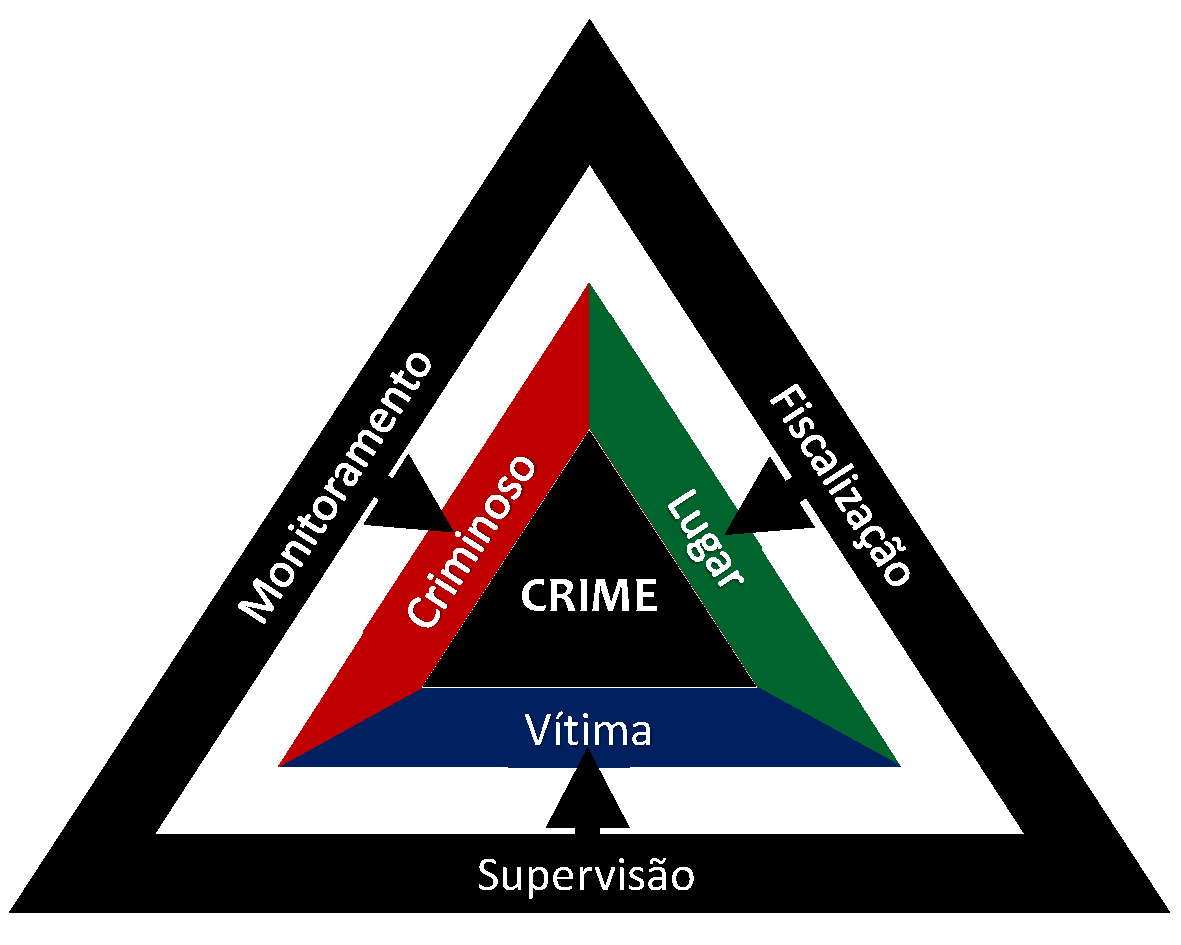
\includegraphics[width=\linewidth]{./Visuais/TrianguloCrime.pdf}
        \end{center}
        \legend{Fonte: Elaborada pelo autor (2020).}
\end{wrapfigure}

O infográfico da \autoref{fig:Crime} apresenta os três elementos básicos da Teoria da Atividade Rotineira, também conhecida como Triângulo do Crime. Em resumo, três elementos são considerados essenciais para a ocorrência de um crime. Para que um crime aconteça deve-se haver um criminoso motivado sem supervisão, um lugar sem fiscalização e uma vítima desprotegida ou vulnerável. Tomar atitudes preventivas sob qualquer um destes elementos, dificulta a ocorrência do crime. Todavia, destaca-se que estes elementos não possuem pesos iguais, mas sim, se interbalanceiam entre si (\textit{e.g.} em certas condições, um lugar bem fiscalizado poderia não ser um empecilho para um criminoso muito motivado).

O Triângulo do Crime apresenta as três partes fundamentais para a ocorrência de um crime. As estratégias de combate ao \ac{ASI} se objetivam a agir sob estas partes fundamentais. Algumas estratégias são focadas no monitoramento de criminosos\footnote{\label{note:nota1}O Canadá conduz um programa comunitário de acompanhamento de infratores sexuais denominado \ac{CoSA}. O programa se objetiva a ajudar e a apoiar agressores sexuais à se reintegrarem à sociedade após cumprirem suas penas de encarceramento. Estudos mostram que o programa é capaz de reduzir em até 80\% a reincidência do crime entre os participantes \cite{wilson2009circles}. Mais informações sobre o programa canadense podem ser acessadas em: \url{https://www.cosacanada.com/}.}, outras no fortalecimento da fiscalização de espaços públicos ou privados\footnote{No Brasil, a lei nº 12.038 visa dificultar a exploração sexual de crianças e adolescentes, ampliando medidas punitivas para os estabelecimentos que hospedarem menores desacompanhados dos pais ou responsáveis, ou sem autorização. Disponível em: \url{http://www.planalto.gov.br/ccivil_03/_Ato2007-2010/2009/Lei/L12038.htm}.}, e outras na capacitação preventiva de potenciais vítimas, tornando-as menos vulneráveis\footnote{A iniciativa educacional \ac{CAPP} busca ensinar crianças à reconhecer, resistir e denunciar abusos. Mais informações sobre o programa podem ser acessadas em: \url{https://www.nyfoundling.org/what-we-do/our-programs/child-welfare/child-abuse-prevention-program-capp/}.}. Cada estratégia pode ser dividida com base em seus níveis de prevenção, podendo ser: prevenção primária, prevenção secundária ou prevenção terciária. Os níveis de prevenção são apresentados em maiores detalhes na \autoref{fig:prevencao}.


\begin{figure}[htb]
	\caption{\label{fig:prevencao}Níveis de Prevenção.}
    \vspace{0.4cm}
    \hspace{-0.75cm}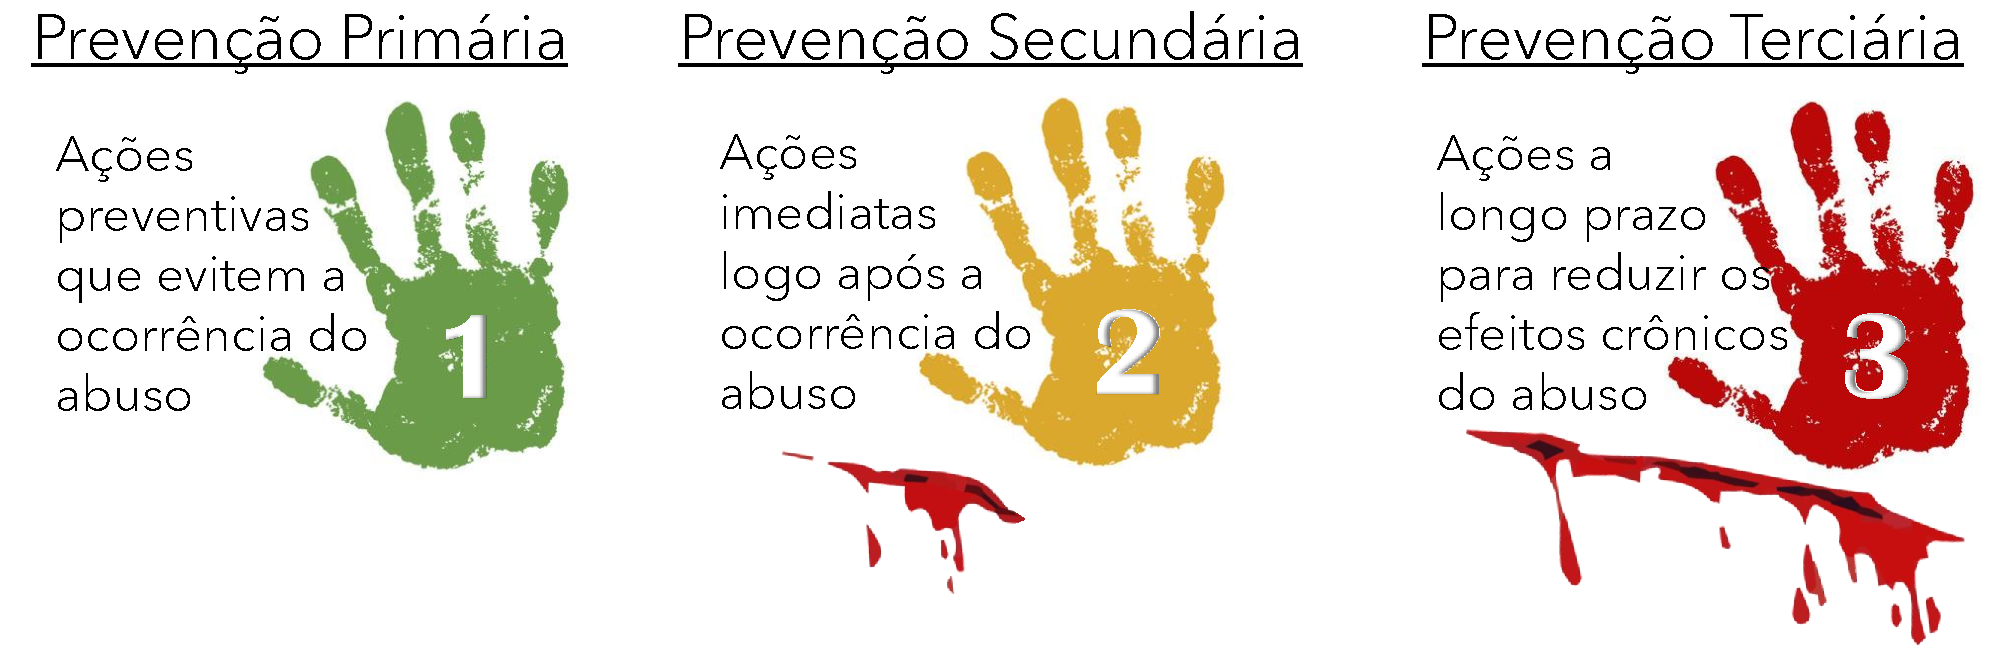
\includegraphics[width=1.1\linewidth]{./Visuais/Prevencao.pdf}

	\legend{Fonte: Elaborada pelo autor (2020).}
\end{figure}

A \autoref{fig:prevencao} apresenta os três níveis de prevenção mais comumente relatados na literatura pesquisada. São eles: prevenção primária, prevenção secundária e prevenção terciária \cite{dahlberg2006violencia, santos2011guia, maria2012abusos, cardoso2015abuso}. No caso do \ac{ASI}, a prevenção primária engloba iniciativas que antecipam a incidência do abuso sexual contra crianças e adolescentes  \cite{marcelino2017vamos}. A prevenção secundária enfatiza uma resposta imediata após a ocorrência da violência sexual. Já a prevenção terciária corresponde, de modo geral, a ações de longo prazo para o tratamento e recuperação das vítimas \cite{escocia2020expert}. Informa-se que a literatura médica relata também um quarto nível de prevenção. A prevenção quaternária descreve sobre ações preventivas contra eventuais exageros na utilização de métodos preventivos \cite{tesser2017importante}. Embora presente na literatura médica, salienta-se que a atual dissertação engloba apenas os três níveis de prevenção mais relatados pela bibliografia pesquisada acerca do abuso sexual de crianças e adolescentes.

Os níveis de prevenção do \ac{ASI} não se resumem a atuar apenas sob as crianças. Há registros de prevenção terciária relacionados inclusive ao tratamento/acompanhamento de agressores sexuais\footref{note:nota1}. O combate ao abuso sexual de crianças e adolescentes assume então inúmeras facetas, cada qual, objetivada a diminuir de alguma forma os fatores de risco que influenciam a ocorrência de violações sexuais.

Os \acfp{FR} são aquelas circunstâncias que aumentam a probabilidade da ocorrência de um episódio de violência. Deste modo, o abuso infantil apresenta mais chances de ocorrer quando os fatores de risco se acumulam. Os \acp{FR} interagem entre si, no que é chamado de risco em cascata, no qual um risco inicial pode acompanhar ou desencadear outros riscos, terminando por resultar em um acúmulo sucessivo de fatores de risco \cite{Recommendations2019Taylor}. A \autoref{fig:Riscos} apresenta a disposição dos fatores de riscos mais apontados pela literatura na área por meio de um Modelo Ecológico. 

\pagebreak

\begin{figure}[htb]

    \caption{\label{fig:Riscos}Modelo Ecológico para a compreensão da violência contra crianças.}
    \hspace{-2.8cm}
    %\begin{center}
      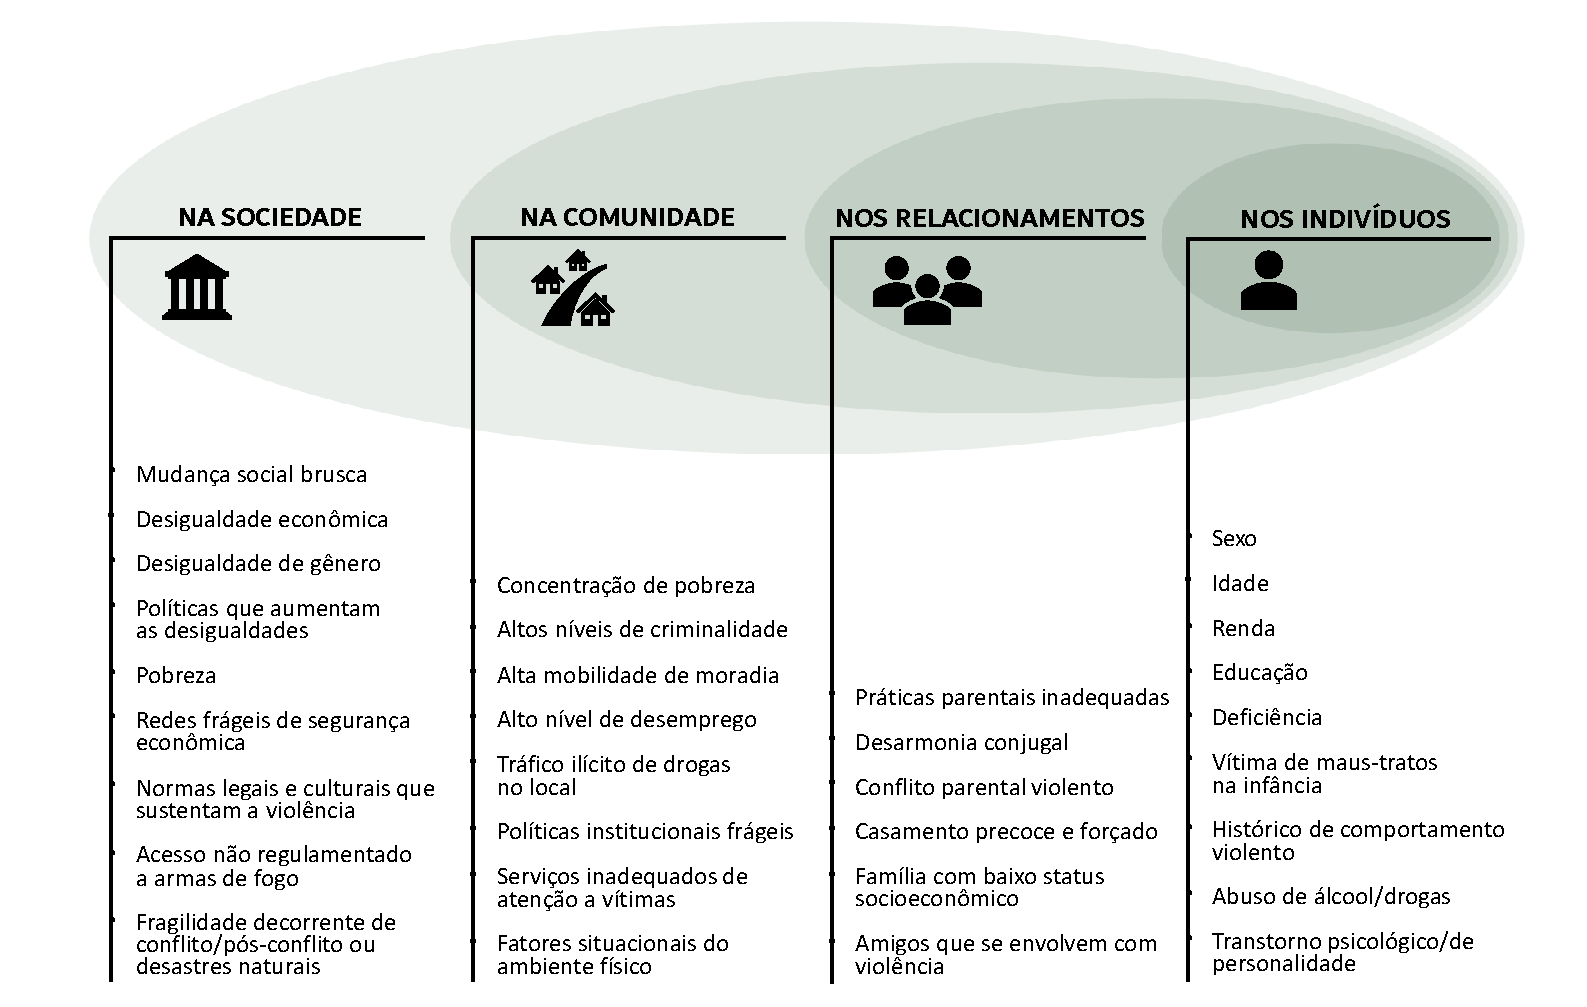
\includegraphics[width=1.28\linewidth]{./Visuais/Ecologico.pdf}
      %\end{center}
    \legend{Fonte: adaptado de \citeonline[p. 17]{inspire2016seven}.}
  
  \end{figure}

O Modelo Ecológico da \autoref{fig:Riscos} ilustra os quatro fatores de risco mais presentes na bibliografia pesquisada. Acentua-se que os fatores de risco podem variar em quantidade e em nomenclatura, dependendo da fonte literária \cite{centers2004sexual, sexual2017department, blasco2018abuso, UNICEF2016promising}. Todavia, a ideia base do Modelo Ecológico tende a permanecer inalterada. O modelo em si, explora a relação entre os fatores individuais e contextuais que acabam por implicar em um cenário de violência \cite{dahlberg2006violencia}. Os fatores de risco do abuso sexual de crianças e adolescentes mais influentes são:

\begin{itemize}
    \item \textbf{Individual:} \hfill Aspectos individuais que fomentem a ocorrência do abuso sexual. %Válido tanto para as vítimas quanto para os agressores. 
    \item \textbf{Relacional:} \hfill Questões familiares que viabilizam as condições para a violência.  %circunstâncias
    \item \textbf{Comunidade:} \hfill Condições econômicas e governamentais que propiciem o abuso.
    \item \textbf{Sociedade:} \hfill Crenças sociais que estimulem atividades sexuais com menores. 
\end{itemize}

Os \acp{FR} podem interatuar entre si de modo a maximizar as chances de um evento abusivo. O baixo nível educacional de um \textbf{Indivíduo} é um dos elementos a ser citado neste aspecto \cite{dahlberg2006violencia}. A negligência da \textbf{Família} nos cuidados infantis é outro aspecto a ser citado \cite{blasco2018abuso}. Cita-se também, a permissividade do casamento infantil de algumas \textbf{Culturas} \cite{bandiera2020women}. Assim, como a baixa condição socioeconômica de uma \textbf{Comunidade}. A exemplo, soros positivos de comunidades africanas veem o relacionamento sexual com crianças como um ato de limpeza e cura da \ac{AIDS} \cite{aded2006abuso}.

Agir sobre os fatores de risco (\autoref{fig:Riscos}), implica em agir de forma mais efetiva no combate a violência sexual infantil. Compreender os níveis de prevenção (\autoref{fig:prevencao}), implica em compreender os momentos de atuar sobre o problema. Entender as raízes da violência (\autoref{fig:Crime}), implica em entender seus elementos operantes. Estudar o problema do \ac{ASI}, é necessário para se ter um panorama geral acerca dos possíveis cenários de atuação e combate. Além disso, um levantamento bibliográfico sobre as estratégias de combate já desenvolvidas se faz indispensável para evitar a perda de tempo e dinheiro no desenvolvimento de uma solução já existente \cite{wazlawick2014metodologia}. 

Este Capítulo elenca as principais soluções utilizadas no combate ao \ac{ASI} de acordo com a bibliografia pesquisada. O levantamento bibliográfico retornou uma quantidade variada de estratégias voltadas ao combate da violência sexual de crianças e adolescentes. Compreender o \textit{modus operandi} de tais estratégias permite identificar as melhores estratégias em termos de custo-benefício. Todavia, embora algumas estratégias possam se ressaltar sobre outras, é importante destacar que o combate a violência sexual de crianças e adolescentes é um esforço multidisciplinar e multissetorial. Sendo assim, é importante ter em mente que as estratégias listadas neste Capítulo não devem ser vistas como concorrentes entre si, mas sim, aliadas na luta e no combate ao \ac{ASI}.

Diante do exposto, a presente dissertação divide as seções deste Capítulo em grupos de soluções utilizadas no combate ao \ac{ASI}. Cada solução visa mitigar o problema da sua própria maneira. Dentre as soluções apresentadas, informa-se que as soluções baseadas em jogos são abordadas a parte (\autoref{ssec:TR}) de forma mais aprofundada e detalhada por se tratarem do cerne da atual pesquisa. Dito isso, a \autoref{sec:regras} descreve normas e legislações sobre os direitos das crianças, a \autoref{sec:canais} apresenta algumas formas de denúncia, a \autoref{sec:propagandas} aponta ações publicitárias, a \autoref{sec:hospital} trata de questões hospitalares, a \autoref{sec:centros} apresenta os centros de atendimento, a \autoref{sec:dp} lista algumas delegacias especializadas, a \autoref{sec:op} elenca operações policiais, a \autoref{sec:infratores} apresenta alguns tratamentos com infratores, a \autoref{sec:programas} menciona alguns programas de capacitação, a \autoref{sec:materiais} relata materiais didáticos de ensino e a \autoref{sec:finais} dá as considerações finais do presente Capítulo. 

%-------------------------------------------------------------------------------------------------------------------

\section{Legislação}\label{sec:regras}

A elaboração de leis e normativas define um instrumento legal para a garantia dos direitos das crianças. Anteriormente a este instrumento legal as crianças não eram consideradas sujeitos de direito \apud{tavares2001direito}{oliveira2017evoluccao}. As cortes judiciais do século XIX enxergavam os relatos de crianças que manifestavam o abuso sexual, como alegações fantasiosas ou mesmo mentirosas \cite{aded2006abuso}. A esperança das crianças de terem suas vozes devidamente ouvidas (e seus direitos assegurados) iria surgir apenas no século XX.

No início do século XX, a sueca Ellen Key manifestou-se sobre o novo século denominando-o como \textbf{Século da Criança} \cite{sandin1999imagens, hayes2002children, junior2016olhares}. Este século marca a fundação da \ac{ONG} \textit{Save the Children}, responsável pela defesa dos direitos da criança no mundo. A fundação data de 1919, anos depois, em 1924 a fundadora da organização Eglantyne Jebb escreveu um documento que seria conhecido mundialmente como a Declaração dos Direitos da Criança de Genebra ou Declaração de Genebra.

A Declaração de Genebra estabelece cinco direitos fundamentais, os quais dão as crianças o direito de serem alimentadas, de serem ajudadas primeiro em caso de catástrofe, de serem escolarizadas, de serem bem tratadas e de serem protegidas contra qualquer forma de exploração. A Declaração dos Direitos da Criança de Genebra destaca-se na história como o primeiro documento internacional voltado a registrar e defender os direitos da criança. Em 1948 os direitos das crianças passaram a ser reconhecidos pela \ac{DUDH}, e pela Declaração dos Direitos da Criança adotada pela \ac{AGNU}, em 1959 \cite{lelis2014fragmentaccao}. Anos depois em 1989, a \ac{ONU} adotou em suas normativas a Convenção sobre os Direitos da Criança, o qual tornou-se o instrumento de direitos humanos mais aceito na história, ratificado ao total por 196 países. 

No Brasil, a história dos direitos das crianças e dos adolescentes começa em 1990, graças ao \acf{ECA}. O Estatuto é considerado um marco na defesa dos direitos da criança e do adolescente brasileiro \cite{lima2012direitos}. Os menores são protegidos pela legislação brasileira contra qualquer forma de negligência, discriminação, crueldade, opressão, violência e exploração. 

A legislação é um instrumento chave na luta contra a violência sexual infantil. Os direitos estabelecidos juridicamente garantem uma maior proteção aos menores. A tipificação de crimes contra as crianças pode desencorajar certos agressores sexuais de praticarem seus delitos. Para os delitos já praticados, a legislação continua sendo um instrumento chave na luta contra a violência sexual infantil, pois além de garantir tratamento as vítimas, assegura o encarceramento do criminoso sexual (\textit{e.g.} a lei nº 12.978, de 21 de maio de 2014, torna hediondo o crime de exploração sexual de crianças e adolescentes, impedindo o condenado de obter anistia, graça ou indulto ou pagar fiança).

%-------------------------------------------------------------------------------------------------------------------

\section{Ouvidorias e Canais de Denúncia}\label{sec:canais}

\begin{wrapfigure}[35]{r}{5.2cm}%pulando 35 linhas
  \vspace{-20pt}
  \caption{\label{fig:Canais}Ouvidorias Infantis.}

  \subfloat[Brasil.\label{fig:Brasil}\vspace{-3pt}]{
\includegraphics[width=\linewidth]{./Visuais/Ouvidorias/100-Brasil.png}}\vspace{1pt}
  \\
  \subfloat[Argentina.\label{fig:Argentina}\vspace{-3pt}]{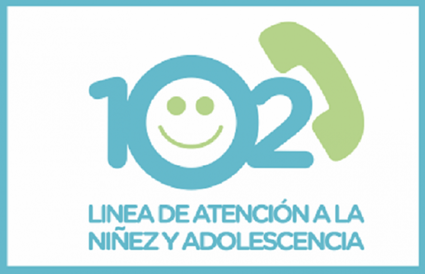
\includegraphics[width=\linewidth]{./Visuais/Ouvidorias/102-Argentina.png}}\vspace{1pt}
  \\
  \subfloat[Vietnã.\label{fig:Vietna}\vspace{-3pt}]{
\includegraphics[width=\linewidth]{./Visuais/Ouvidorias/111-Vietna.png}}\vspace{1pt}
  \\
  \subfloat[França.\label{fig:Franca}\vspace{-3pt}]{
\includegraphics[width=\linewidth]{./Visuais/Ouvidorias/119-Franca.png}}\vspace{1pt}
  \\
  %\subfloat[Aruba\label{fig:Aruba}\vspace{-3pt}]{
\includegraphics[width=\linewidth]{./Visuais/Ouvidorias/131-Aruba.png}}\vspace{1pt}
  \\
  \subfloat[Japão.\label{fig:Japao}\vspace{-3pt}]{
\includegraphics[width=\linewidth]{./Visuais/Ouvidorias/189-Japao.png}}\vspace{1pt}
  \\
  \subfloat[Índia.\label{fig:India}\vspace{-3pt}]{
\includegraphics[width=\linewidth]{./Visuais/Ouvidorias/1098-India.png}}\vspace{1pt}
  \\
  \subfloat[Tailândia.\label{fig:Tailandia}\vspace{-3pt}]{
\includegraphics[width=\linewidth]{./Visuais/Ouvidorias/1387-Thailandia.png}}\vspace{1pt}
  %\begin{center}
  %  
\includegraphics[width=\linewidth]{./Visuais/Ouvidorias/100-Brasil.png}
  %\end{center}
  %\begin{center}
  %  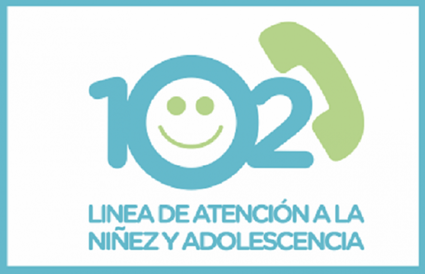
\includegraphics[width=\linewidth]{./Visuais/Ouvidorias/102-Argentina.png}
  %\end{center}
  %\begin{center}
  %  
\includegraphics[width=\linewidth]{./Visuais/Ouvidorias/131-Aruba.png}
  %\end{center}
  %\begin{center}
  %  
\includegraphics[width=\linewidth]{./Visuais/Ouvidorias/111-Vietna.png}
  %\end{center}
  %\begin{center}
  %  
\includegraphics[width=\linewidth]{./Visuais/Ouvidorias/189-Japao.png}
  %\end{center}
  %\begin{center}
  %  
\includegraphics[width=\linewidth]{./Visuais/Ouvidorias/1098-India.png}
  %\end{center}
  %\begin{center}
  %  
\includegraphics[width=\linewidth]{./Visuais/Ouvidorias/1387-Thailandia.png}
  %\end{center}
  %\begin{center}
  %  
\includegraphics[width=\linewidth]{./Visuais/Ouvidorias/119-Franca.png}
  %\end{center}
  \legend{Fonte: \citeonline{UNICEF2017new}.}%eu paguei outros nao citados aqui, como fazer a referencia?
  %india (mas não governamental)
\end{wrapfigure}

Os canais de denúncia são uma estratégia relevante no combate a violência sexual infantil. Os meios de comunicação para delação servem de alicerce para garantir os direitos legalmente estabelecidos das crianças e dos adolescentes. Entre os meios de denúncia mais amplamente presentes pelo mundo estão as linhas telefônicas. A \autoref{fig:Canais} elenca as principais ouvidorias telefônicas de alguns países.

Os números telefônicos da \autoref{fig:Canais} demonstram a preocupação dos países em garantir um canal seguro de comunicação para crianças em situação de risco. A depender do país, cada canal de comunicação pode aceitar outras formas de denúncia, além da violência infantil. No caso do Brasil, o Disque 100 (\autoref{fig:Brasil}), além de receber denúncias contra crianças, também recebe denúncias de outros grupos vulneráveis como idosos e deficientes. Os meios de denúncia veem no intuito de mitigar as lacunas deixadas pelas políticas públicas no que diz respeito a fiscalização.

Os canais telefônicos são instrumentos de denúncia a distância confiáveis e acessíveis \cite{UNICEF2017new}. A penetrância dos dispositivos móveis no Brasil, torna este instrumento ainda mais poderoso no combate à violência infantil, uma vez que a quantidade de dispositivos móveis operantes no país ultrapassa a própria população brasileira. Além das denúncias por ouvidorias telefônicas, as denúncias podem ser realizadas por correio eletrônico, aplicativos e portais governamentais. As denúncias no Brasil podem ser realizadas de forma totalmente gratuita durante toda a semana 24 (vinte e quatro) horas por dia (incluindo sábados, domingos e feriados).

Os canais de denúncia fortalecem as políticas públicas de enfrentamento e combate a violência sexual infantil. As linhas de atendimento infantil permitem que crianças e jovens encontrem um caminho para sua segurança e bem-estar. Os canais de denúncia são fontes confiáveis e acessíveis para ajudar e apoiar crianças e jovens em situação de risco, além de encaminhá-los para os devidos sistemas nacionais de proteção a infância e a adolescência \cite{UNICEF2017new}.

%-------------------------------------------------------------------------------------------------------------------

\section{Canais de Divulgação}\label{sec:propagandas}

Os canais de divulgação são indispensáveis para a disseminação de informações substanciais para se combater à violência sexual infantil. Os meios de divulgação ajudam na dispersão do conhecimento e na conscientização da população. Os programas de conscientização da população são largamente conhecidos por auxiliarem suas respectivas lutas. %seja em capampanhas de vacinação ou em campanhas de combate a mosquitos transmissores de doenças. 
No caso da violência sexual infantil, ações publicitárias auxiliam as crianças sobre seus direitos ensinando-as e encorajando-as a realizarem denúncias. Um exemplo de ação publicitária neste estilo é apresentado na \autoref{fig:ad}.

\begin{figure}[htb]%
  \centering
  \caption{\label{fig:ad}Propaganda de consientização contra a violência sexual infantil.}%
  \subfloat[\centering \label{fig:adulto}Propaganda na visão do Adulto.]{{\frame{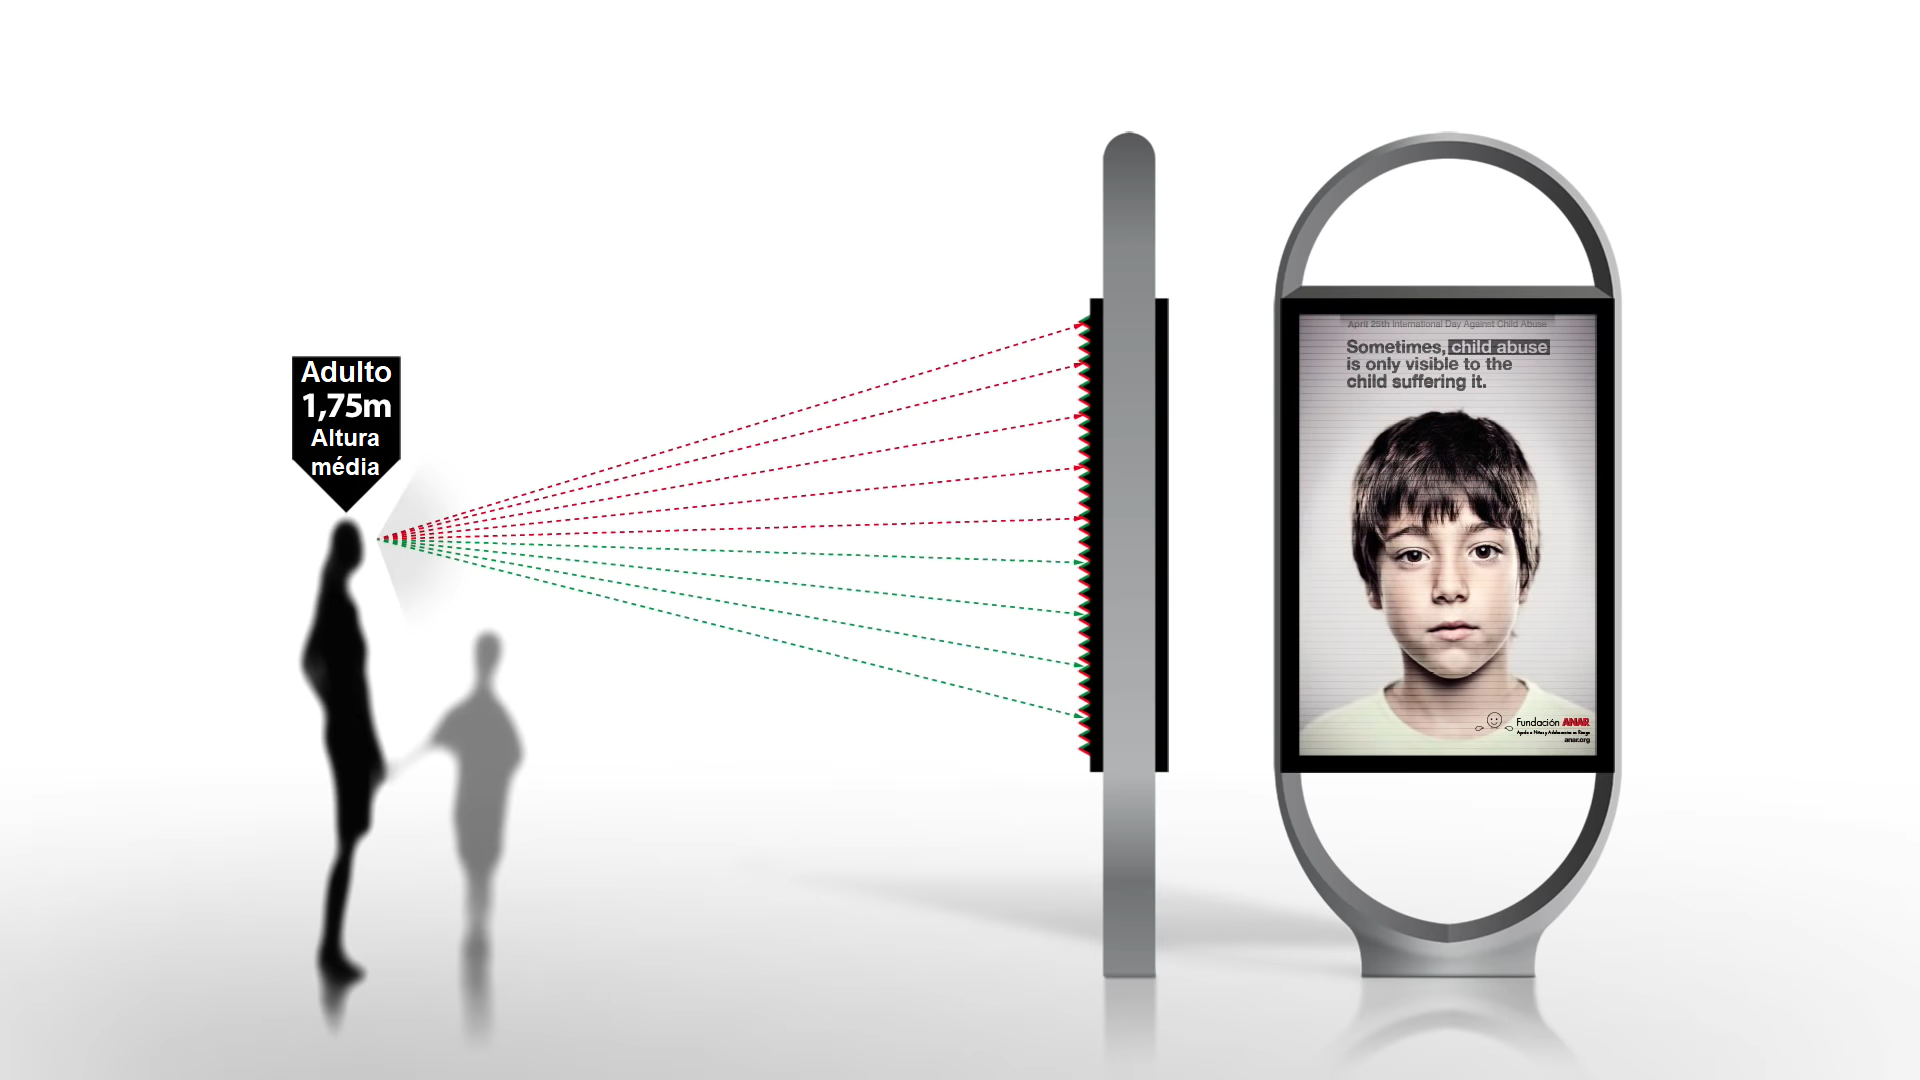
\includegraphics[width=0.48\linewidth]{./Visuais/Propagandas/Propaganda-Adulto.png}}}}%
  \hspace{0.01cm}
  \subfloat[\centering \label{fig:crianca}Propaganda na visão da Criança.]{{\frame{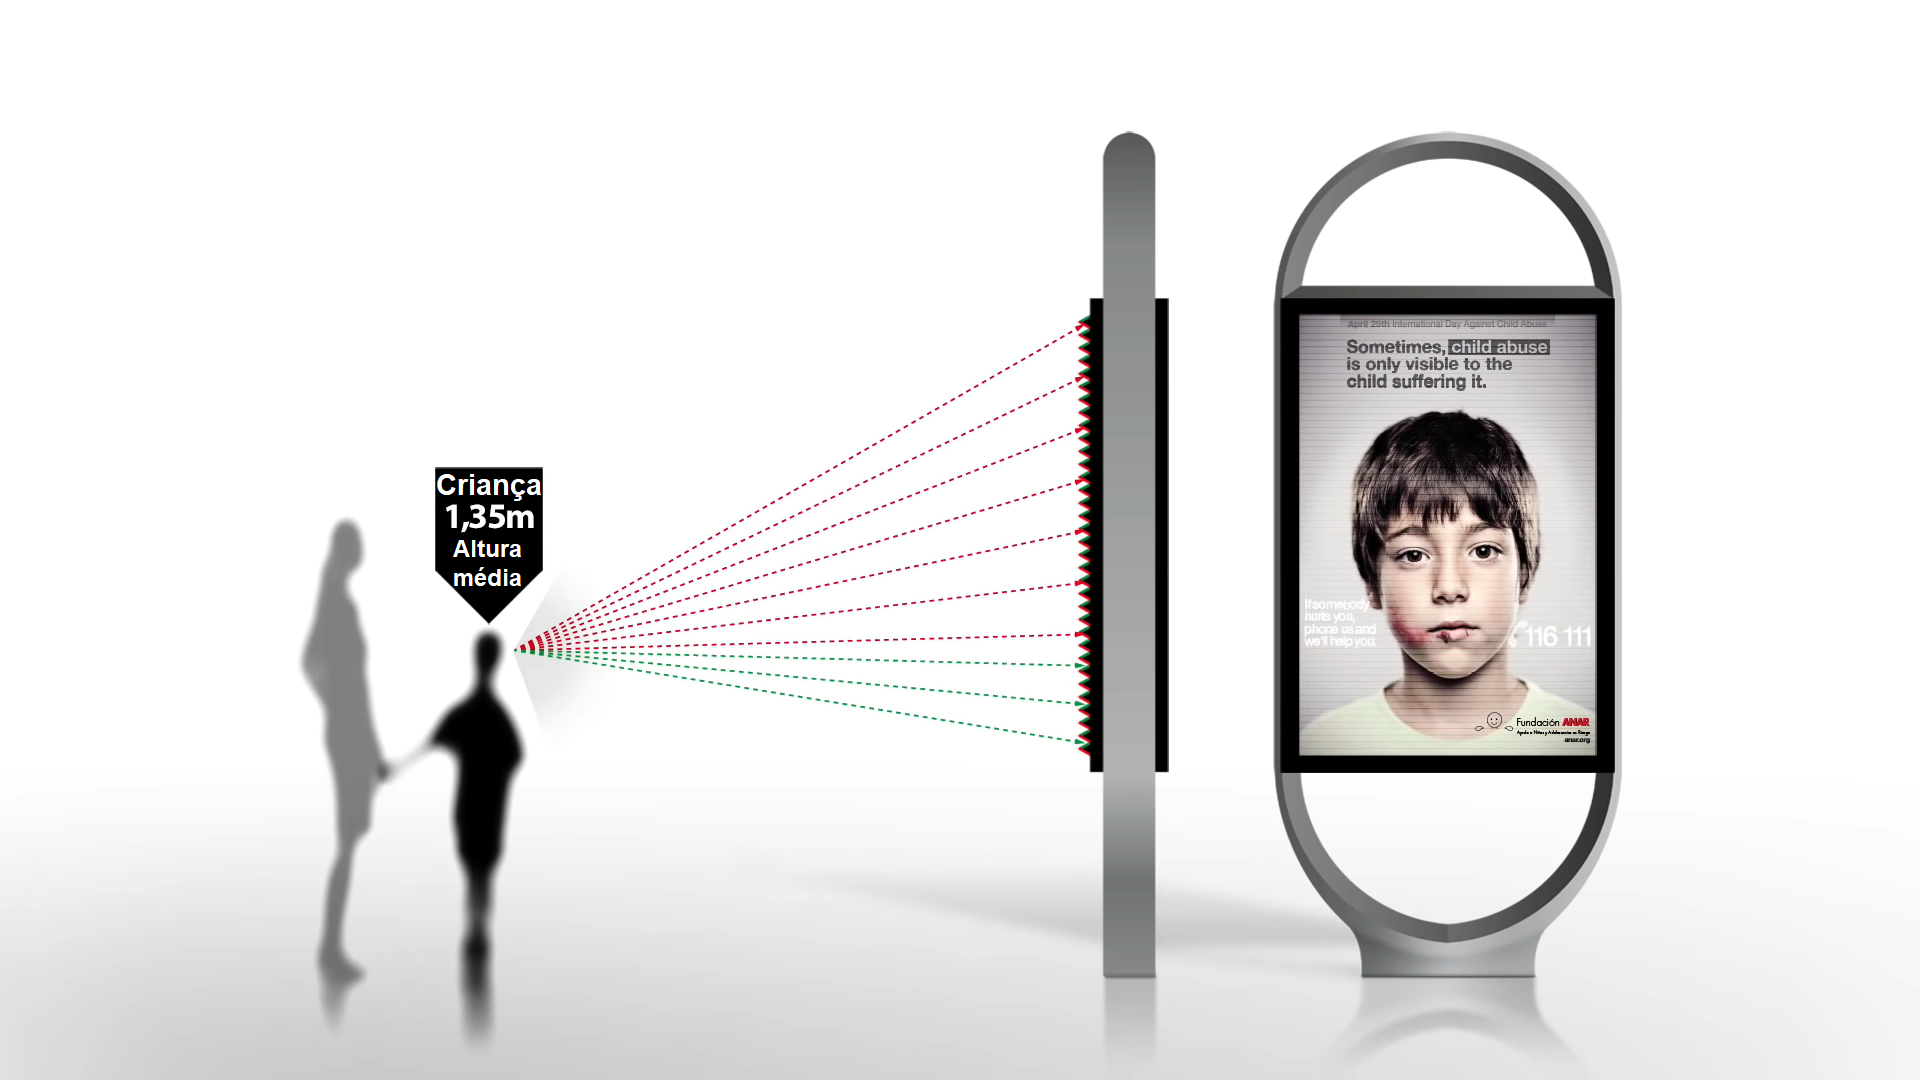
\includegraphics[width=0.48\linewidth]{./Visuais/Propagandas/Propaganda-Crianca.png}}}}%
  \vspace{10pt}
  \legend{Fonte: adaptado de \citeonline{anar2013campana}.}
  \label{fig:example}%
\end{figure}

A \autoref{fig:adulto} e a \autoref{fig:crianca} apresentam a mesma propaganda, porém vista de ângulos diferentes. A propaganda parte da concepção de que muitas crianças violentadas transitam pelas ruas com seus próprios agressores. Agressores estes, que para não serem encarcerados garantem o desconhecimento da criança sobre os meios de denúncia relativos ao crime cometido. A propaganda então, baseada sob estes princípios, apresenta uma mensagem visível apenas a partir do ângulo de visão da altura média de uma criança (1,35 metros). A mensagem, dentre outras informações, apresenta aos menores um número telefônico, o qual permite um canal de ajuda e socorro as crianças vítimas de violência. 

As ações publicitárias auxiliam na divulgação de informações, as quais capacitam as pessoas a reconhecerem o problema e a reagirem adequadamente ao problema. Os meios de divulgação são os mais variados, podendo ir desde comerciais no rádio, na televisão ou na \textit{internet} \cite{martinez2000prevencion}. Além disso, excelentes meios de divulgação são cartazes, panfletos, cartilhas e campanhas governamentais \cite{mendelson2015parent}. A divulgação de informação deve ser capaz de atingir a massa da população para que resulte em um impacto significativo a nível social. Não foram encontrados dados a nível nacional sobre o aumento de denúncias de violência sexual após determinada campanha. No entanto, do ponto de vista individual, a extensão dos meios de divulgação possibilita que indivíduos em situação de risco possam vir a conhecer melhor sobre seus direitos. Desta forma, os meios de comunicação se assentam como uma peça-chave na luta contra os maus-tratos infantis. 

%-------------------------------------------------------------------------------------------------------------------

\section{Atendimento Hospitalar}\label{sec:hospital}

Os atendimentos hospitalares são procedimentos poderosos no combate aos maus-tratos contra as crianças. O profissional de saúde surge como um sujeito ativo, no sentido de identificar abusos e denunciá-los, conforme ordena a legislação brasileira \cite{Lei:8069:1990, almeida2012responsabilidade, costa2019maus}. Inúmeros jornais e portais de notícias já relataram inclusive o diagnóstico de violência sexual infantil em laudos médicos\footnote{Portal de Notícias G1 (08/08/2019): \url{https://g1.globo.com/sp/sao-jose-do-rio-preto-aracatuba/noticia/2019/08/08/pais-tiram-crianca-de-hospital-antes-de-alta-apos-medico-suspeitar-de-sinais-de-abuso-sexual.ghtml}.}\footnote{Redação de Notícias Catve.com (28/12/2018): \url{https://catve.com/noticia/9/238135/menina-de-11-anos-e-internada-com-dores-abdominais-e-medico-descobre-gravidez}.}\footnote{Portal de Notícias G1 (08/08/2018): \url{https://g1.globo.com/ro/ji-parana-regiao-central/noticia/2018/08/08/mae-leva-filha-de-5-anos-ao-pediatra-e-descobre-que-menina-foi-estuprada-em-ro.ghtml}.}\footnote{Rede Jornalística A Gazeta (03/11/2017): \url{https://www.gazetaonline.com.br/noticias/policia/2017/11/menino-contrai-sifilis-e-familia-descobre-abuso-sexual-1014106068.html}.}\footnote{Portal de Notícias G1 (12/09/2016): \url{http://g1.globo.com/mato-grosso/noticia/2016/09/crianca-de-1-ano-morre-em-hospital-e-medicos-denunciam-suposto-abuso.html}.}\footnote{Jornal Metropóles (07/06/2016): \url{https://www.metropoles.com/distrito-federal/seguranca-df/medico-denuncia-estupro-de-menina-de-11-anos-em-festa-de-escola-no-df}.}\footnote{Portal de Notícias G1 (26/08/2015): \url{http://g1.globo.com/sao-paulo/itapetininga-regiao/noticia/2015/08/mae-descobre-que-filho-foi-estuprado-apos-dentista-achar-doenca-na-boca.html}.}\footnote{Portal de Notícias G1 (23/04/2013): \url{http://g1.globo.com/sp/bauru-marilia/noticia/2013/04/exame-aponta-que-menina-de-3-anos-sofreu-abuso-sexual-em-bauru-sp.html}.}.

A literatura médica comenta sobre a dificuldade em constatar sinais de violência infantil em alguns casos. Em certas circunstâncias se exige do médico muito mais perspicácia e experiência profissional \cite{paiva2012violencia}. Devido a complexidade no diagnóstico de alguns episódios de abuso, guias clínicos foram desenvolvidos como o Guia Clínico da \aclu{OMS} \cite{OMS2017responding}. Os relatórios e guias médicos são capazes de ajudar os profissionais de saúde a identificar mais facilmente sinais de abuso acometidos contra a criança e contra o adolescente \cite{christian2015aap}.

Os guias e relatórios médicos ajudam tanto no diagnóstico, quanto na procedência dos tramites legais. Nos casos agudos e recentes de violência sexual, as medidas legais já devem acompanhar toda a assistência inicial de diagnóstico e tratamento. Nos casos crônicos e repetitivos, sem grandes lesões visíveis, deve-se realizar o registro de anamnese, histórico familiar e dados de exame físico. Além disso, é fundamental a realização de um \ac{B.O.} em uma delegacia de polícia, para fins de processo judicial e para a comprovação da agressão, bem como para confecção de exames e investigações que levem à identificação devida do agressor \cite{paiva2012violencia}. 

O atendimento hospitalar adiciona mais uma camada de defesa no enfretamento a violência sexual infantil. Embora os abusos só possam ser diagnosticados após sua ocorrência, a defesa médica ainda se faz válida para diminuir a reincidência dos eventos abusivos, seja em um exame de rotina ou qualquer outra forma de atendimento \cite{costa2019maus}.

%-------------------------------------------------------------------------------------------------------------------

\section{Centros de Tratamento às Vítimas}\label{sec:centros}

Os centros de tratamento estabelecem uma poderosa estratégia de enfretamento ao maltrato infantil. No Brasil, o tratamento e recuperação da criança vítima de violência pode ser executado tanto pelo Conselho Tutelar, quanto pelo \ac{CREAS}. Os centros de tratamento surgem sob uma perspectiva de fornecer suporte e apoio necessário a indivíduos em situação de risco, tal como garantir seus direitos legalmente estabelecidos \cite{caccia2014conselheiros}.

O Conselho Tutelar é um órgão permanente e autônomo, não jurisdicional, encarregado de zelar pelo cumprimento dos direitos da criança e do adolescente \cite{brasil2002notificacao}. Já o \ac{CREAS}, é responsável pelo acolhimento e pelo atendimento a famílias e indivíduos em situação de risco pessoal e social, por violência, abuso e exploração sexual, ocorrência de abandono, maus-tratos físicos e/ou psíquicos, cumprimento de medidas socioeducativas, situação de rua e de trabalho infantil, entre outras situações de violação dos direitos.

No que tange a violência sexual infantil, os centros de tratamento operam de modo a recuperar a saúde física e mental das crianças e dos adolescentes acometidos por essa forma de violência. Os menores são ouvidos e encaminhados aos seus devidos cuidados. Esse processo possibilita menores chances de revitimização desses indivíduos, diminuindo assim as taxas de violência sexual de crianças e adolescentes \cite{faraj2016atendimento}. A implementação de centros de tratamento estabelece um grande aliado na proteção dos direitos da infância e da juventude e a sua implementação no país é de extrema importância para enfrentar o problema da violência sexual contra crianças e adolescentes. 

O Conselho Tutelar não presta o atendimento direto às vítimas de violência, mas atua de forma que ele se viabilize em casos concretos de ameaça ou violação de direitos. A legislação brasileira informa inclusive que os casos de suspeita ou confirmação de maus-tratos contra criança ou adolescente devem, obrigatoriamente, ser comunicados ao Conselho Tutelar da respectiva localidade, sem prejuízo de outras providências legais. Em adendo, a lei obriga que exista pelo menos um Conselho Tutelar por município composto de pelo menos cinco membros com idoneidade moral escolhidos pela comunidade local. 

O tratamento devido, de crianças e adolescentes, vítimas de violência sexual é crucial para mitigar os males causados por essa forma de violência. Ou seja, os centros de tratamento às vítimas não almejam enfrentar diretamente a questão dos maus-tratos de crianças e adolescentes, mas sim, os problemas gerados por esses maus-tratos, tais como: depressão, estresse pós-traumático e ideação suicida. Desta forma, os cuidados tomados com crianças e adolescentes vem de modo a ajudá-los a superar suas sequelas físicas ou psicológicas. Em adendo, essa política pública de tratamento ainda é capaz de estabelecer uma estratégia válida para diminuir a reincidência de eventos abusivos \cite{costa2019maus}.

%-------------------------------------------------------------------------------------------------------------------

\section{Departamentos Policiais}\label{sec:dp}

As delegacias especializadas são um bom artifício de confronto a violência sexual infantil. No Brasil, a competência para fiscalizar, investigar e instaurar inquérito e procedimentos policiais nos casos de infração penal praticada contra crianças e adolescentes é realizada pelas polícias civis. As polícias civis são de responsabilidade dos estados, sendo assim, sua estrutura organizacional e processual varia a depender da região do país \cite{rodrigues2014violencia}. Não há uma diretriz operacional única entre as delegacias especializadas a nível nacional. Algumas delegacias ficam abertas 24 (vinte e quatro) horas por dia, todos os dias da semana, enquanto outras operam apenas nos dias úteis e em horário comercial. E mesmo as abertas 24 (vinte e quatro) horas não possuem uma equipe multidisciplinar de plantão, contando com apenas os funcionários essenciais para o registro da ocorrência como agentes, escrivães e delegado \cite{brasil2016estudo}.

As delegacias especializadas no atendimento de crianças e adolescentes se dividem em duas categorias. As voltadas para o atendimento aos menores vítimas de violência e as voltadas para lidar com os menores infratores. Salienta-se que existem delegacias que conjugam essas duas funções em um mesmo órgão. Além dessa diferença legal, as delegacias podem divergir em sua estrutura no que diz respeito a presença ou não de carceragem, brinquedoteca e salas de atendimento psicológico \cite{brasil2016estudo}. Em adendo, algumas delegacias relataram inclusive convênios com hospitais, universidades e \acfp{ONG}. No entanto, independente da delegacia, todas integram o \ac{SGDCA}.

O \ac{SGDCA} compreende principalmente: os centros de defesas, as delegacias especializadas, as varas da infância e juventude, as promotorias da infância e juventude e os Conselhos Tutelares \cite{rodrigues2014violencia}. Fazer parte do \ac{SGDCA}, implica que os órgãos associados devem conferir máxima prioridade ao atendimento das crianças na faixa etária da primeira infância com suspeita ou confirmação de violência de qualquer natureza, formulando projeto terapêutico singular que inclua intervenção em rede e, se necessário, acompanhamento domiciliar. Isso faz com que todas as delegacias especializadas tenham uma estrutura em comum que atenda devidamente a esses requisitos. 

As delegacias especializadas assentam uma excelente estratégia de socorro policial aos menores sexualmente violentados. O atendimento policial ao menor vítima de violência produz uma resposta ao problema semelhante as respostas dos centros de tratamento. Contudo, as delegacias especializadas estabelecem um combate mais direto ao problema ao conduzir um processo legal para a devida identificação e apreensão do agressor. Tal ação é capaz de reduzir a quantidade de indivíduos potencialmente perigosos em circulação na sociedade, garantido assim a diminuição na incidência de eventos envolvendo a violência sexual de crianças e adolescentes. 

%-------------------------------------------------------------------------------------------------------------------

\section{Operações Policiais}\label{sec:op}

As operações policiais são excelentes alternativas na luta contra o abuso, o tráfico e a exploração sexual infantil. No Brasil e no mundo as operações são responsáveis pela busca e apreensão de inúmeros criminosos sexuais, o que acaba por mitigar a reincidência do crime por parte destes agressores.

A literatura relata a Operação Carrossel (2007) como o primeiro esforço policial internacional a combater a pornografia infantil na \textit{internet} \cite{lowenkron2014all}. Todavia, há registros anteriores que relatam a mesma abrangência policial internacional, como a Operação Catedral (1998) objetivada também no combate a pornografia infantil na \textit{internet} \cite{barrot2008brochuras, jesus2006anti}. É importante destacar que isto não se trata necessariamente de uma contradição literária, a Operação \textit{Darknet} (2014) também é descrita como pioneira no combate a distribuição de material pornográfico infanto-juvenil na \textit{internet}, contudo o pioneirismo desta, configura-se pela metodologia de investigação e pelas ferramentas para identificar usuários criminosos na \textit{Deep Web} \cite{tonello2018pedofilia}. Ou seja, cada operação pode ser classificada como pioneira com base em seus contextos específicos. 

No Brasil, o \ac{MJ} considera a Operação Luz na Infância (2017) como a maior operação de enfretamento a pornografia infantil no Brasil e na América Latina. Isto, pois a operação é um conglomerado de vários países e instituições \cite{souza2018sabemos}. Entre os países estão: Brasil, Chile, El Salvador, Equador, Estados Unidos da América, Panamá e Paraguai. A Operação Luz na Infância já teve mais de 7 (sete) fases, as quais já apreenderam um volume total de dados que ultrapassa os 3 (três) \aclu{TB}, além da prisão de mais de 500 (quinhentos) indivíduos. 

As operações policiais são políticas públicas de segurança que estão fundamentadas e baseadas nos limites da legislação e da jurisdição de suas nações, resguardados os acordos internacionais. Dito isso, é notória a dependência que as operações policiais possuem com o âmbito jurídico. Se não há tipificação legal do crime, então não a crime a ser reprimido. Por tal razão que a sansão de decretos e a criação de leis neste contexto se fazem fundamentais para o fortalecimento das operações policiais. 

A dependência jurídica das operações policiais pode ser uma barreira a ser enfrentada no combate a violência sexual infantil. De nada adianta uma operação contra o abuso de crianças em um país que permite legalmente o casamento infantil. Além da barreira jurídica, as estratégias policiais sofrem do mesmo mal dos atendimentos hospitalares, uma vez que a apreensão do criminoso só pode ocorrer após a ocorrência do crime ou a tentativa dê, todavia a defesa policial ainda se faz válida para diminuir a reincidência dos eventos abusivos uma vez que os criminosos tenham sido encarcerados ou levados a tratamento. 

%-------------------------------------------------------------------------------------------------------------------

\section{Gestão de Infratores}\label{sec:infratores}

O encarceramento de criminosos sexuais é uma boa alternativa de combate ao problema da violência sexual infantil, no curto prazo. O encarceramento de agressores sexuais remove indivíduos perigosos do convívio social, além de trazer conforto e tranquilidade às suas vítimas. No entanto, o encarceramento não resolve a questão da violência sexual de crianças e adolescentes, no longo prazo.  

Há longo prazo, os agressores sexuais apresentam taxas de reincidência elevadas após sua soltura. A explicação, vem da ausência de intervenções dirigidas à problemática, durante o cumprimento da pena de prisão \cite{ribeiro2018programas, finkelhor2009prevention, maia2014castraccao}. A atitude unicamente punitiva de sistemas jurídicos, acaba por não tratar devidamente o problema do abuso sexual \cite{camila2019violencia}. Embora a atração sexual por crianças e adolescentes seja considerada uma patologia, o agressor sexual não é considerado inimputável perante a justiça, caso o delito tipificado em lei seja cometido \cite{ribeiro2018programas}. Contudo, um tratamento adequado ao agressor se faz necessário para diminuir a probabilidade da reincidência do crime. Os programas de tratamento apresentam uma taxa de sucesso alta, implicando assim em uma baixa reincidência dos crimes sexuais \cite{ribeiro2018programas}. Meta-análises apoiam inclusive os efeitos significativos de tratamentos baseados em princípios cognitivo-comportamentais \cite{mendelson2015parent}.

As terapias e os tratamentos aos agressores sexuais precisam ser realizados com muita cautela. Por mais que os delitos cometidos pelos agressores sexuais sejam desumanos e atentem contra o livre direito de suas vítimas; por questões éticas ainda se faz necessário garantir que os tratamentos e que as terapias não violem os direitos dos agressores sexuais \cite{finkelhor2009prevention}. Por tal razão terapias de aversão, choque ou tratamentos de castração química não são recomendadas por algumas instituições de saúde \cite{maia2014castraccao}. Expressar empatia e compreensão com as pessoas que cometeram violência sexual frequentemente é visto como se a atitude do abusador fosse defendida (o que é errôneo). Especialistas defendem que a humanização do agressor seja feita para a condução de um tratamento mais adequado.

A literatura relata tanto tratamentos voltados aos já infratores, quanto tratamentos voltados aos indivíduos não incidentes que são sexualmente atraídos por crianças, e que buscam ajuda para lidar melhor com sua patologia sexual \cite{finkelhor2009prevention}. Esforços de ambos os gêneros produzem efeitos promissores relatados por alguns estudos na área \cite{mendelson2015parent}.

O tratamento de indivíduos sexualmente atraídos por crianças pode ajudar que não haja novas vítimas e para que aqueles que já cometeram algum crime, não voltem a fazê-lo. Demonstram-se como um excelente meio de resolução do problema, pois o problema não é resolvido pura e simplesmente com a punição do agressor, mais sim, com o seu tratamento. 

%-------------------------------------------------------------------------------------------------------------------

\section{Programas de Capacitação}\label{sec:programas}

Os programas de capacitação demonstram-se como uma excelente alternativa para o enfrentamento aos maus tratos contra os menores. O processo de capacitação busca instruir determinados indivíduos sobre um certo âmbito. No caso da violência infantil, de modo geral os programas buscam ensinar um conjunto de indivíduos a identificar e reagir adequadamente ao problema. 

Os processos de capacitação podem envolver desde uma grande comunidade até grupos específicos de indivíduos. Neste sentido, a atual seção apresenta os três grupos mais corriqueiramente relatados pela literatura na área: os pais/responsáveis das crianças (\autoref{ssec:pais}), os profissionais que trabalham com crianças (\autoref{ssec:professores}) e as próprias crianças (\autoref{ssec:alunos}).

\vspace{1.0 cm}
\subsection{Pais/Responsáveis}\label{ssec:pais}

Os programas sobre sexualidade para pais/responsáveis buscam, no geral, conscientizá-los sobre os cuidados necessários para que suas crianças tenham um risco menor de sofrer qualquer tipo de violência sexual \cite{pelisoli2010prevenccao}. Essa conscientização pode vir por meio de programas voltados para a instrução de pais/responsáveis, ou de projetos voltados para a conscientização de pais/responsáveis a respeito dos programas infantis. 

Os programas voltados a instrução de pais/responsáveis se baseiam em preencher algumas lacunas de conhecimento, trazendo assim, mais informações no âmbito da violência infantil para pais ou responsáveis \cite{maria2010papel}. A ideia de tais programas é desmistificar alguns mitos relacionados a temática da violência sexual infantil, assim como fornecer informação adequada, recursos práticos e dar apoio.

Os projetos voltados para a conscientização de pais/responsáveis a respeito dos programas infantis estão normalmente associados a programas de educação em sexualidade para crianças. Muitos guardiões legais se preocupam com os programas preventivos de cunho sexual ministrados as suas crianças, pois temem que estes programas possam levar as crianças a saberem muito sobre sexo, depravando-as de alguma forma \cite{chen2007prevention}. Sendo assim, os projetos de conscientização para pais/responsáveis vêm no intuito de prestar esclarecimento de modo a tornar os programas de educação sexual para crianças menos restritivos. 

Programas parentais sobre sexualidade demonstram resultados promissores na redução dos maus-tratos infantis \cite{silverman2008evidence}. Embora os dados indiquem que a maior parte dos maus-tratos de crianças e adolescentes advém dos próprios responsáveis legais da criança, os programas ainda se fazem válidos para aqueles que buscam trazer maior segurança e proteção para suas crianças \cite{pelisoli2010prevenccao}.

\subsection{Profissionais}\label{ssec:professores}

Treinar profissionais que trabalham com crianças para o reconhecimento e enfretamento do \ac{ASI} é uma boa estratégia para se combater a violência contra as crianças. Entre os profissionais a serem treinados estão principalmente os: médicos, professores e policiais. Os médicos são treinados a diagnosticarem de forma mais rápida e adequada os casos de violência infantil \cite{paiva2012violencia}. Os professores são ensinados de modo a torná-los mais comprometidos com os programas de educação sexual para crianças \cite{colleen2016advancing}. Já os policiais são instruídos a agir de maneira efetiva as denúncias realizadas \cite{pelisoli2010prevenccao}. 
%os próprios gestores reconhecem o despreparo dos profissionais, a precariedade de recursos, a ineficiência dos encaminhamentos e a falta de articulação entre diferentes setores que atuam nessa área. \cite{pelisoli2010prevenccao}
Um programa que abrange esses três tipos de profissionais é o Programa Criança Protegida. 

O Programa Criança Protegida tem o objetivo de capacitar conselheiros tutelares, agentes de saúde, policiais, guardas municipais, professores e outros profissionais ligados à garantia dos direitos da criança e do adolescente no enfrentamento de violações, principalmente os crimes de abuso sexual contra vulneráveis \cite{oei2020tomada}. Infelizmente, o alcance bibliográfico da atual pesquisa não foi capaz de encontrar estudos conclusivos que atestassem a eficácia do treinamento de todos estes profissionais no combate ao abuso infantil. Todavia, falando especificamente dos profissionais ligados a educação, pesquisas já confirmam a eficácia no treinamento de professores ligados a programas de educação sexual infantil \cite{colleen2016advancing}. 

\subsection{Alunos}\label{ssec:alunos}

A educação sexual infantil é uma boa forma de prevenir a violência sexual de crianças e adolescentes \cite{finkelhor2009prevention}. Os programas preventivos para crianças buscam educar os menores a reconhecerem e a responderem adequadamente a episódios abusivos, evitando assim, que a violência aconteça. Os programas educacionais para a prevenção da violência sexual infantil podem abranger desde as crianças da mais tênue idade até adolescentes quase entrando em sua vida adulta. Os programas voltados a educar as menores faixas etárias são os mais criticados, por responsabilizarem demasiadamente a criança \cite{colleen2016advancing}. Nesses programas, existe a preocupação da criança culpar a si mesma após um episódio de violência, por não ter evitado o abuso, possivelmente agravando ainda mais os traumas deixados no menor. Existem outras críticas feitas a tais programas, devido a sua temática sensível e delicada \cite{scholes2014serious}. Todavia os programas educacionais para crianças estão entre as melhores iniciativas de combate à violência infantil \cite{barron2008school, finkelhor2009prevention}.

A eficiência dos programas infantis na prevenção da violência sexual, advém de um fato conhecido na história da área. Historicamente, sabe-se que os agressores sexuais preferem atuar sobre crianças com menores chances de manifestarem resistência aos seus abusos, tais crianças são classificadas pelos agressores sexuais como sendo a \textit{vítima ideal} \cite{budin1989sex}. Portanto, a instrução e capacitação de crianças nessa temática diminui a quantidade de \textit{vítimas ideais} presentes na sociedade, coibindo assim, os predadores sexuais de praticarem seus delitos.


\section{Materiais de Ensino}\label{sec:materiais} 

Os materiais de ensino são grandes aliados do processo pedagógico. Os materiais englobam no geral, toda a classe de dispositivos e utensílios que auxiliam a obtenção de conhecimento sobre um determinado assunto. No âmbito da violência infantil, os materiais de ensino funcionam como ótimas ferramentas de reforço aos ensinos preventivos da área. A prevenção nesse sentido, pode ser atingida através do estudo individual dos materiais ou através do seu uso em programas educacionais infantis (como forma de complemento aos programas).

Os materiais didáticos vêm de modo a aprimorar o processo pedagógico. Os materiais funcionam não apenas como um instrumento facilitador do aprendizado infantil, mas também como uma ferramenta de auxílio aos professores. Entre os materiais didáticos de maior predominância ao longo da história, estão os livros.

Programas baseados em livros de educação sexual infantil, permitem a visualização mais acurada e precisa dos conceitos ensinados, na mesma medida que proporcionam listas de exercícios e atividades para o fortalecimento de tais conceitos \cite{maria2010papel}. O aprendizado pode ser complementado não apenas com livros, mas também com vídeos.

Os vídeos são ótimos materiais de ensino pois, diferentemente dos livros, proporcionam um conteúdo dinâmico com fluidez e movimentação, o que acaba por fortalecer o processo pedagógico \cite{maria2010papel}. Há ainda o fato de que os vídeos abrem um canal sonoro de comunicação, aumentando assim a retenção e a aprendizagem. No âmbito sonoro, salienta-se também a utilização de músicas no contexto da prevenção à violência sexual infantil.

Diferente dos livros e dos vídeos, as músicas são normalmente mais utilizadas em terapias para o tratamento de crianças violentadas. Terapias musicais estão relacionadas com uma autoimagem mais positiva e um melhor desenvolvimento da autoestima. O processo terapêutico com auxílio de músicas é capaz de ajudar as crianças a se sentirem melhor com elas mesmas, ajudando-as assim, em sua recuperação \cite{robarts2003healing}. Além das músicas, dos vídeos e dos livros ainda é possível citar os jogos de tabuleiro como um material de apoio a educação preventiva da violência sexual (os jogos digitais são abordados separadamente no \autoref{ssec:TR}).

Jogos de carta, tabuleiro e até mesmo atividades em papel, são utilizados como um instrumento lúdico na aprendizagem infantil. O ambiente recreativo dos jogos permite que assuntos sensíveis e delicados possam ser abordados de maneira mais divertida e natural. Devido a essas características, especialistas consideram as abordagens educativas baseadas em jogos extremamente benéficas para o ensino preventivo da violência sexual \cite{meyer2017analise}.

%Jogos de um modo geral são capazes de fortalecer o processo pedagógico. Os jogos são uma via que possibilita que assuntos difíceis, sensíveis ou embaraçosos possam ser abordados de uma forma lúdica, permitindo a diversão associada a aprendizagem \cite{stieler2016paper}. 

Os materiais de ensino se estabelecem como boas estratégias no combate à violência sexual de crianças e adolescentes. Livros, vídeos, músicas e jogos são capazes de educar crianças e jovens a se protegerem de eventuais episódios de abuso. Para os abusos já consumados, tais materiais ainda se estabelecem como fortes aliados para a realização de denúncias e para o tratamento das vítimas. 

%-------------------------------------------------------------------------------------------------------------------

\section{Considerações Finais}\label{sec:finais}

As estratégias elencadas por esse Capítulo são iniciativas que surgiram como resposta ao problema da violência sexual de crianças e adolescentes. Cabe destacar que todas as iniciativas aqui apresentadas advêm de inúmeras fontes literárias. Não há portanto, uma única fonte de pesquisa citada por este trabalho que agrega todas as soluções aqui apresentadas. Um compilado de todas as iniciativas apresentadas neste Capítulo é ilustrado no infográfico da \autoref{fig:Metodos}.

\vspace{0.5cm}

\begin{figure}[htb]
	\caption{\label{fig:Metodos}Principais Métodos de Combate ao Problema do Abuso Sexual Infantil.}\vspace{0.4cm}
  %\begin{adjustwidth}{-4.2cm}{-0.0cm}
    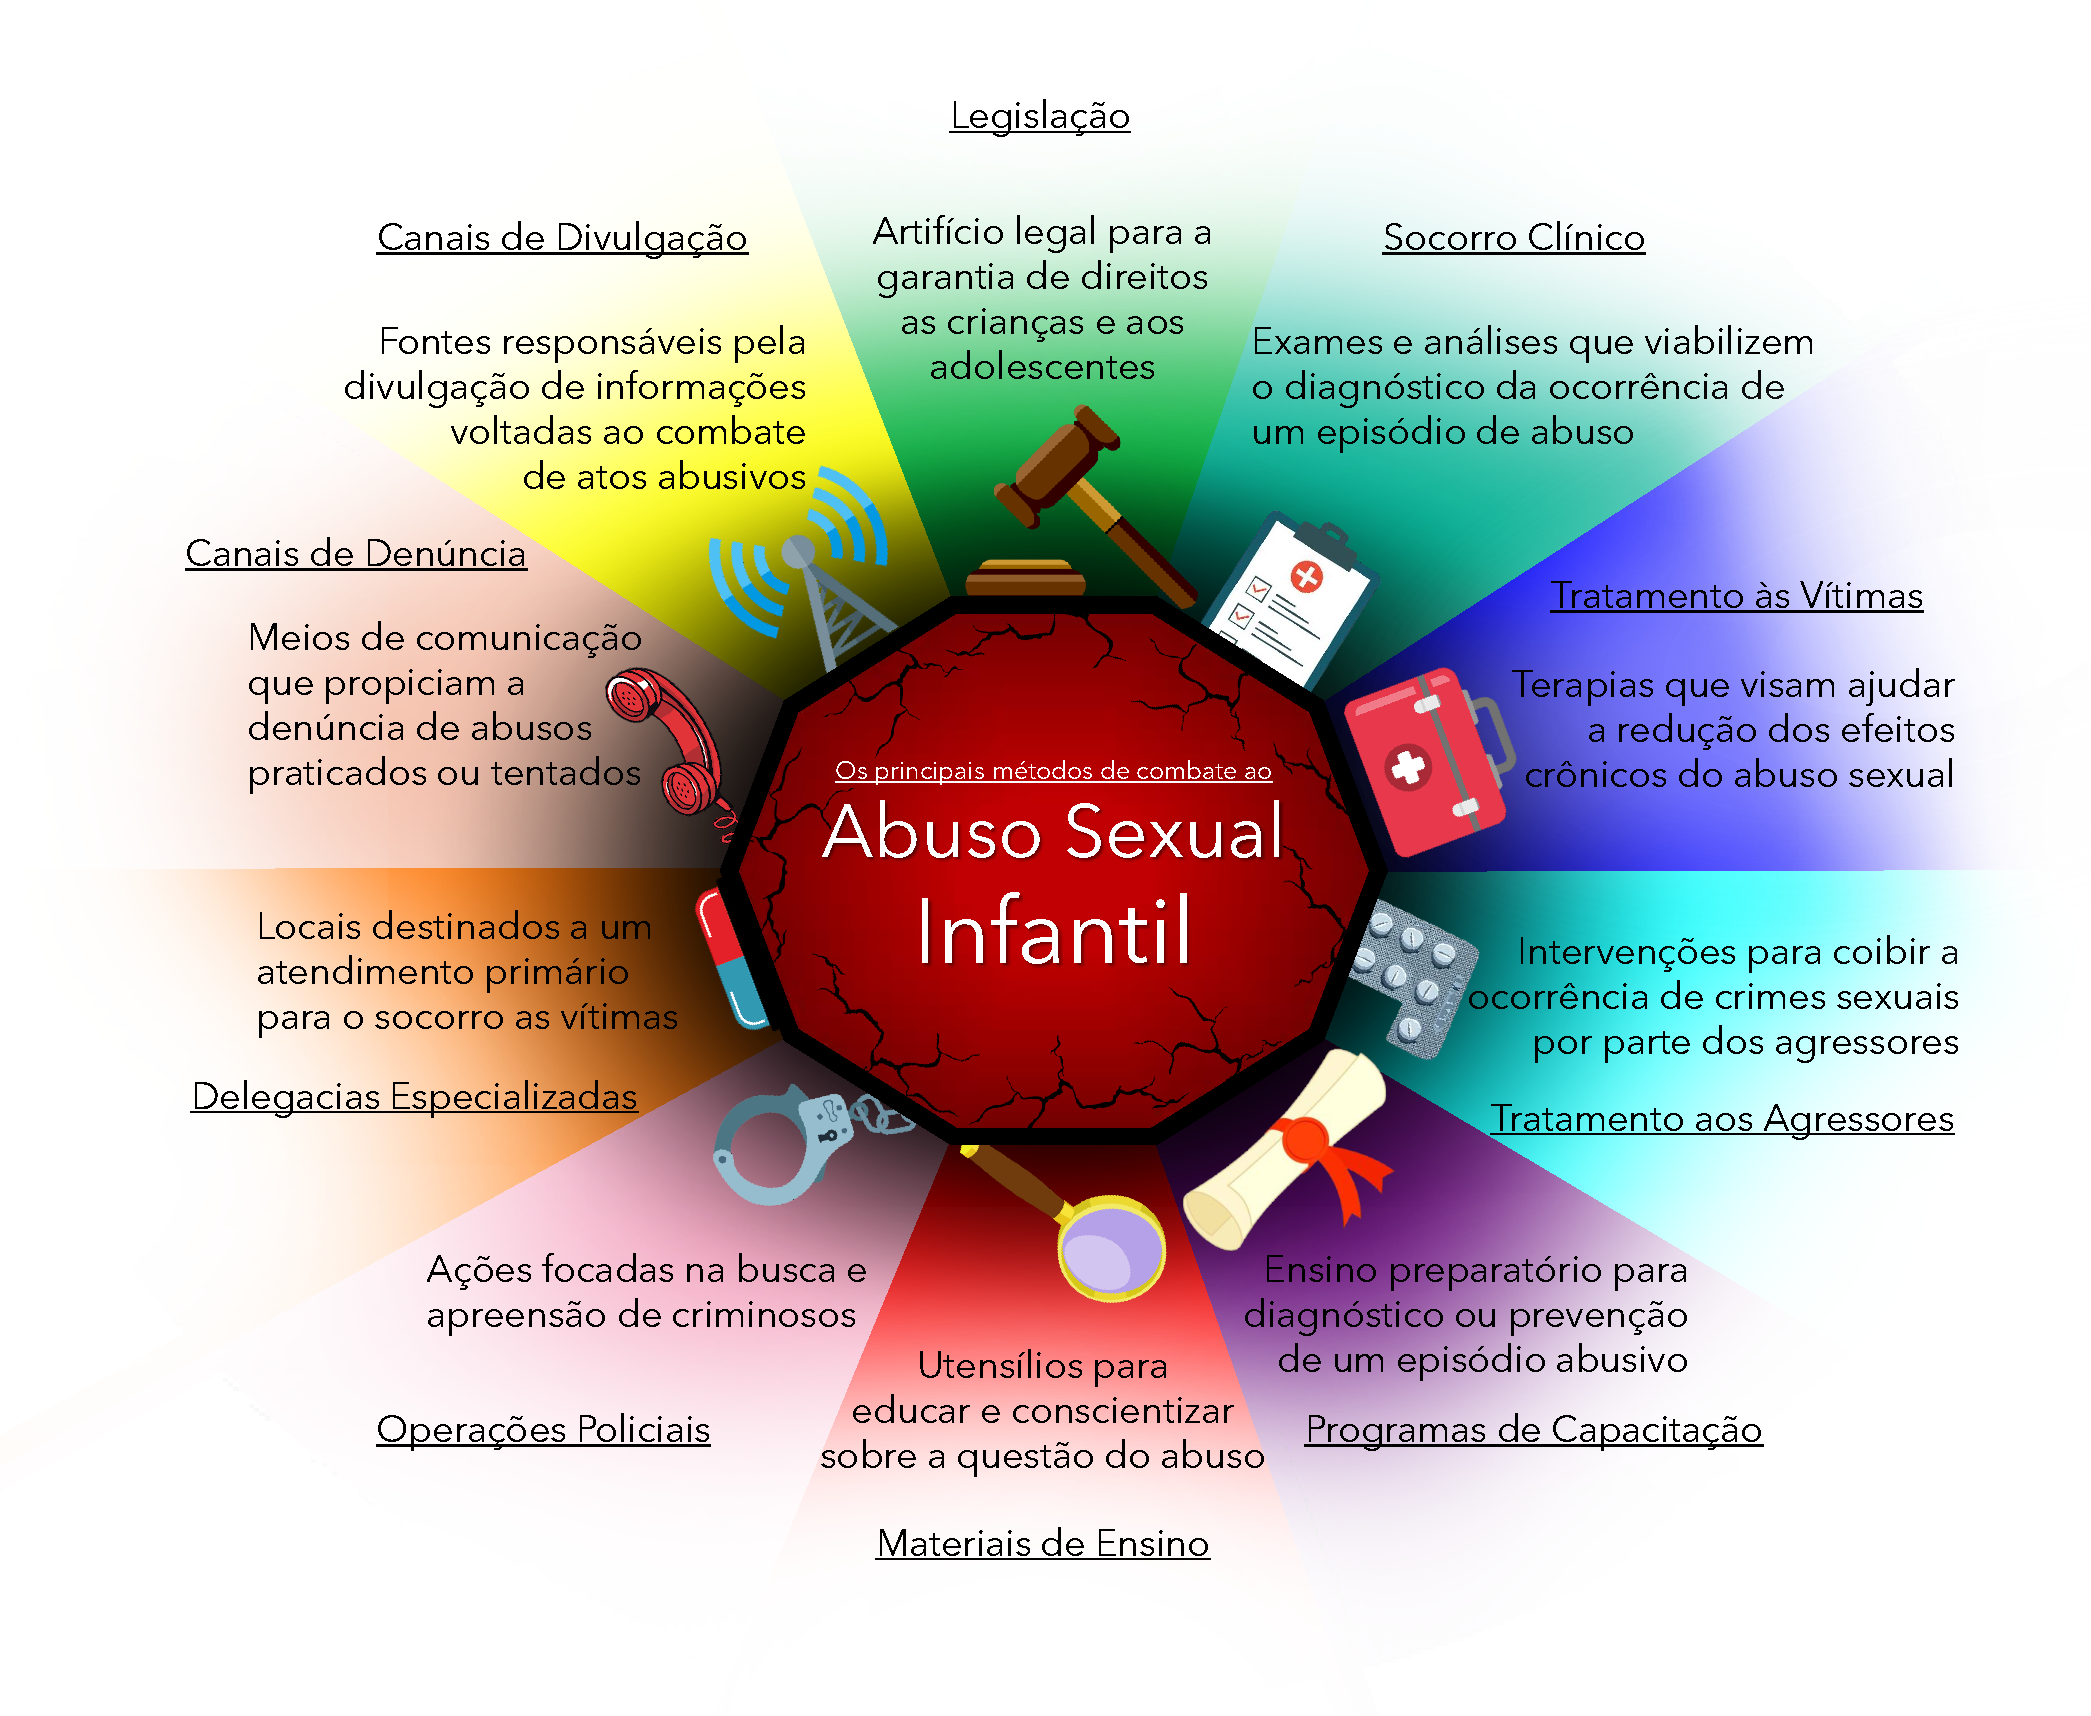
\includegraphics[width=\linewidth]{./Visuais/MétodosCombate.pdf}
	%\end{adjustwidth}\vspace{-1.0cm}
  \legend{Fonte: Elaborada pelo autor (2020).}
\end{figure}

A \autoref{fig:Metodos} ilustra as estratégias de combate à violência sexual infantil apresentadas neste trabalho. No âmbito jurídico foram criadas medidas legislativas (\autoref{sec:regras}), focadas no fortalecimento dos artifícios legais para o combate a violência sexual de crianças e adolescentes, dentre estes artifícios legais cita-se a criação de inúmeros meios para a denúncia de criminosos (\autoref{sec:canais}). Para conscientizar as pessoas de seus direitos e dos meios de denúncia, surgiram os canais de divulgação (\autoref{sec:propagandas}). Aos já molestados, medidas surgiram em resposta, voltadas ou ao diagnóstico clínico (\autoref{sec:hospital}) ou ao tratamento das vítimas (\autoref{sec:centros}). Na esfera policial foram criadas as delegacias de atendimento (\autoref{sec:dp}) e as operações policiais (\autoref{sec:op}) que acabam por fornecerem uma resposta de combate direta ao problema da violência sexual infantil. Para os infratores, surgiram iniciativas voltadas ao seu tratamento (\autoref{sec:infratores}). No aspecto socioeducativo foram criados programas de capacitação (\autoref{sec:programas}), os quais podem ser complementados por materiais de ensino (\autoref{sec:materiais}), proporcionando assim, um sistema educativo capaz de conscientizar as pessoas sobre a violência sexual de crianças e adolescentes. 

A violência sexual infantil é um grave problema presente na sociedade. Em resposta a este problema sugiram inúmeras medidas nas mais diversas áreas. Por tal razão, este é o tipo de crime que não pode ser abordado numa perspectiva individual, mas sim, abordado em um contexto interdisciplinar e intersetorial \cite{maria2010papel, pinto2017avaliaccao}. É importante que as estratégias de combate à violência sexual infantil estejam em sincronia para terem seus resultados positivos maximizados. O trabalho conjunto das estratégias de combate ao abuso sexual de crianças possibilita uma tática sólida de enfrentamento ao problema, a qual é capaz de minimizar os fatores de risco para a ocorrência do problema (\autoref{fig:Riscos}), a qual é capaz de agir diretamente nos elementos de maior influência para a incidência do crime (\autoref{fig:Crime}), e a qual, é capaz de atuar em todos os instantes do crime (\autoref{fig:prevencao}).

As estratégias elencadas por esse Capítulo não representam a totalidade de estratégias existentes nesse cenário de combate à violência sexual infantil. Soluções muito abrangentes ou soluções muito vagas não foram apresentadas neste trabalho. O agrupamento de soluções, aqui apresentado, é uma visão pessoal do autor dessa dissertação e portanto, única na literatura. O agrupamento realizado dá ênfase aos critérios que nomeiam uma determinada solução, elencando seus principais achados e atestando seu êxito conforme as pesquisas na área apontam.

As estratégias de combate à violência sexual infantil podem ser agrupadas de inúmeras formas. Não há registros na literatura especializada que apontem para um agrupamento único e consolidado de estratégias. Todavia, existem propostas de agrupamentos, diferentes do agrupamento apresentado neste trabalho, constituídos inclusive, por estratégias aqui não listadas. Para uma melhor compreensão da temática tratada por esta pesquisa; a leitura desses agrupamentos e compilados de estratégias é mais do que recomendada: \citeonline{australia2000preventing}, \citeonline{sanderson2004child}, \citeonline{finkelhor2009prevention} e \citeonline{inspire2016seven}.

%-------------------------------------------------------------------------------------------------------------------

\chapter{Trabalhos Relacionados}\label{ssec:TR}

\acfp{JS} são utilizados no processo ensino-pedagógico desde o início da década de \citeyear{clark1970serious}. A partir da década de \citeyear{clark1970serious}, diversos estudos foram conduzidos de modo a identificar os reais impactos que tais jogos tinham no ensino infantil e juvenil \cite{stieler2016paper}. Ao longo dos anos, cientistas e pesquisadores concluíram que a utilização de jogos em sala de aula desencadeava um aumento expressivo no desempenho escolar dos estudantes \cite{wentzel1998social}. O aumento se acentuava mais nas disciplinas relacionadas, de alguma forma, aos conteúdos ministrados pelo jogo. A utilização de jogos em sala de aula é capaz de amplificar os efeitos da aprendizagem escolar \cite{jones2020serious}. Contudo, mesmo com os jogos apresentando resultados positivos na aprendizagem infantil, \acp{JS} ainda apresentam baixas taxas de uso no ensino didático das crianças e dos adolescentes. 

A baixa adoção dos jogos no ambiente escolar pode assumir três causas. A primeira está relacionada com a inexistência de jogos apropriados a uma determinada disciplina. A segunda está ligada com a inaptidão de alguns professores em incorporar os jogos a seus planos de ensino. E a terceira está associada com a falta de equipamentos apropriados nas escolas \cite{colleen2016advancing}. Há ainda uma quarta causa impeditiva relacionada diretamente aos jogos de temática preventiva a violência sexual infantil. No caso, a temática sensível e os tabus sociais que permeiam tais jogos acabam por dificultar sua adoção em salas de aulas \cite{chen2007prevention}. Estes fatores acabam por dificultar a adoção de jogos de caráter educativo no processo de ensino, o que poderia explicar o baixo número de \acp{JS} retornados durante a execução da etapa bibliográfica deste trabalho.

Ao se tratar de jogos voltados para prevenção da violência sexual infantil, a literatura pesquisada revela uma quantidade simplória de jogos relacionados a essa temática. Desta quantidade, poucos são os jogos que foram validados por um processo rigoroso de análise e experimentos acadêmicos \cite{colleen2016advancing}. Sendo assim, poucos são os jogos capazes de atestar cientificamente resultados positivos relacionados a aprendizagem e a diminuição das taxas de violência sexual de crianças \cite{jones2010being}.

O atual Capítulo dá ênfase aos três jogos de maior relevância identificados de acordo com a literatura pesquisada. Deste modo, a \autoref{sssec:Being} aborda sobre o jogo \textit{Being Safety Smart}, a \autoref{sssec:Orbit} discorre sobre o jogo \textit{Orbit Rescue} e a \autoref{sssec:CeS} discute sobre o jogo \textit{Cool and Safe}. Tais jogos se destacam também por utilizarem o questionário \ac{CKAQ} em seus experimentos, possibilitando que uma comparação mais acurada entre as pesquisas possa ser realizada. Desta forma, a \autoref{sssec:finais} realiza um breve comparativo entre tais jogos. Por fim, a \autoref{sssec:outros} lista outros jogos na mesma temática com menor rigor científico, além de dar as conclusões finais do presente Capítulo. 

%-------------------------------------------------------------------------------------------------------------------

\section{Being Safety Smart}\label{sssec:Being}

\textit{Being Safety Smart}\footnote{\textit{Being Safety Smart} é um jogo  da Universidade de Sunshine Coast lançado em fevereiro de 2009. No momento da redação deste trabalho o portal do jogo encontra-se fora do ar. No entanto a página virtual do jogo ainda pode ser acessada por meio de bibliotecas digitais voltadas a manter um acervo de páginas públicas do mundo virtual. Para ter acesso ao jogo basta recorrer a uma destas bibliotecas digitais e pesquisar pelo antigo portal do jogo: \url{http://www.beingsafetysmart.com.au}.} é um jogo digital projetado para combater o sequestro e a violência sexual de crianças. O jogo é voltado para crianças de 6 (seis) a 8 (oito) anos. O jogo almeja capacitar as crianças de modo que elas respondam adequadamente ao problema da violência sexual infantil \cite{jones2008online}. Para isso, o jogo aborda o problema do abuso e do sequestro de crianças por meio de oito níveis distintos voltados para o fortalecimento da segurança pessoal das crianças. Os oito níveis são ministrados unicamente em língua inglesa, os quais podem ser visualizados na tela principal do jogo, ilustrada na \autoref{fig:BSS1}. 

\begin{figure}[htb]
  %\vspace{-0.5cm}
	\caption{\label{fig:BSS1}Tela Principal do jogo \textit{Being Safety Smart}.}
  \begin{center}\vspace{-0.3cm}
    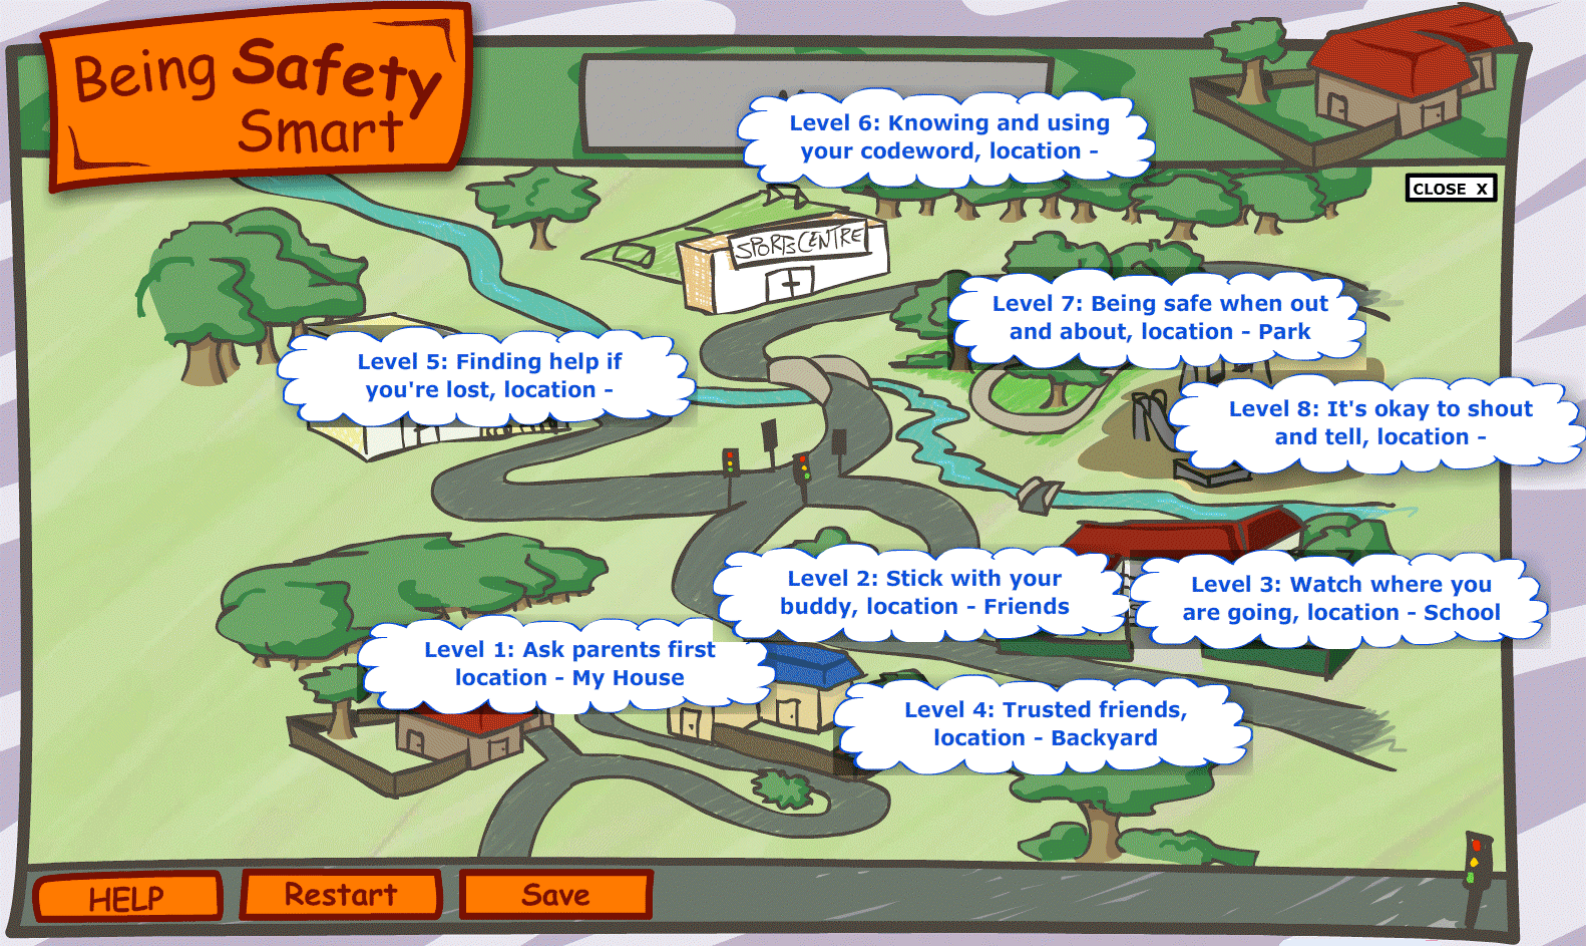
\includegraphics[width=\linewidth]{./Visuais/BSS/B1.png}
	\end{center}\vspace{-0.2cm}
  \legend{Fonte: \citeonline[p. 3]{jones2008online}}
\end{figure}

\vspace{-0.3cm}

A \autoref{fig:BSS1} apresenta a tela principal do jogo \textit{Being Safety Smart}. Oito níveis com diferentes conteúdos didáticos são mostrados nesta tela. Cada nível assume a representação de um ambiente do mundo real. O ambiente representado se relaciona de alguma forma com os assuntos a serem ministrados no nível correspondente. O primeiro nível é ministrado em um ambiente virtual que visa representar a casa da criança, o segundo nível a casa dos amigos da criança, o terceiro nível a escola da criança, o quarto nível a vizinhança da criança, o quinto nível um supermercado, o sexto nível uma quadra esportiva, o sétimo nível um parque e o oitavo nível um pátio recreativo.


\begin{wrapfigure}[39]{r}{3.8cm}%pulando 39 linhas
  \vspace{-5pt}
  \caption{\label{fig:NiveisBBS}Níveis.}
  \vspace{-4pt}
  \subfloat[Nível 1.\label{fig:1}\vspace{-5pt}]{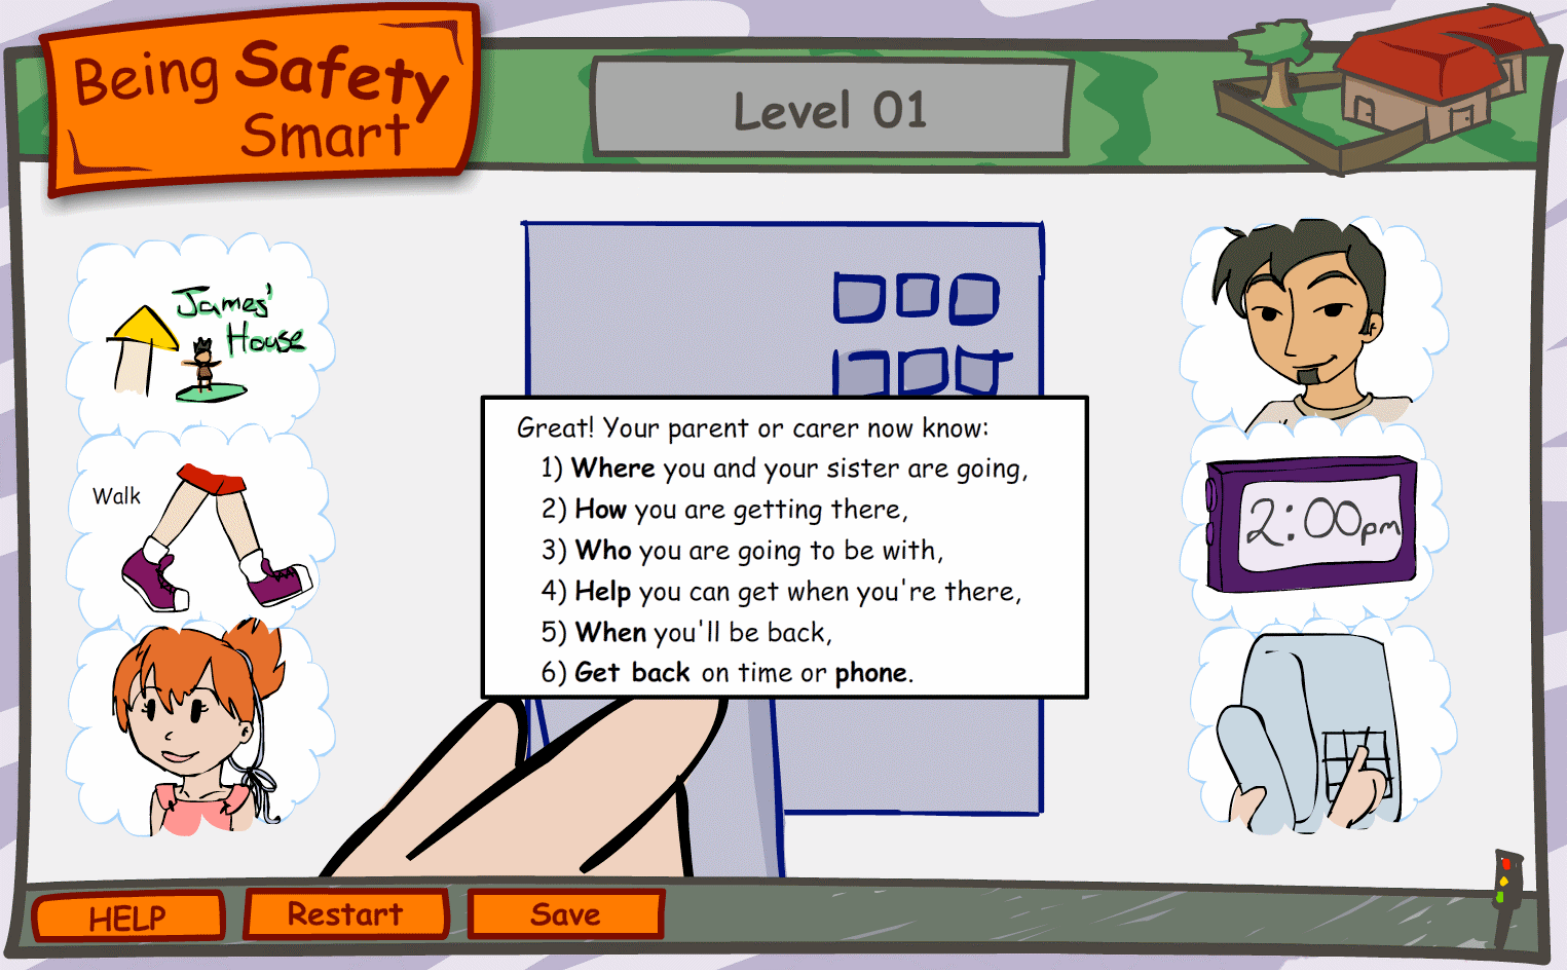
\includegraphics[width=\linewidth]{./Visuais/BSS/B5.png}}\vspace{-3pt}
  \\
  \subfloat[Nível 2.\label{fig:2}\vspace{-5pt}]{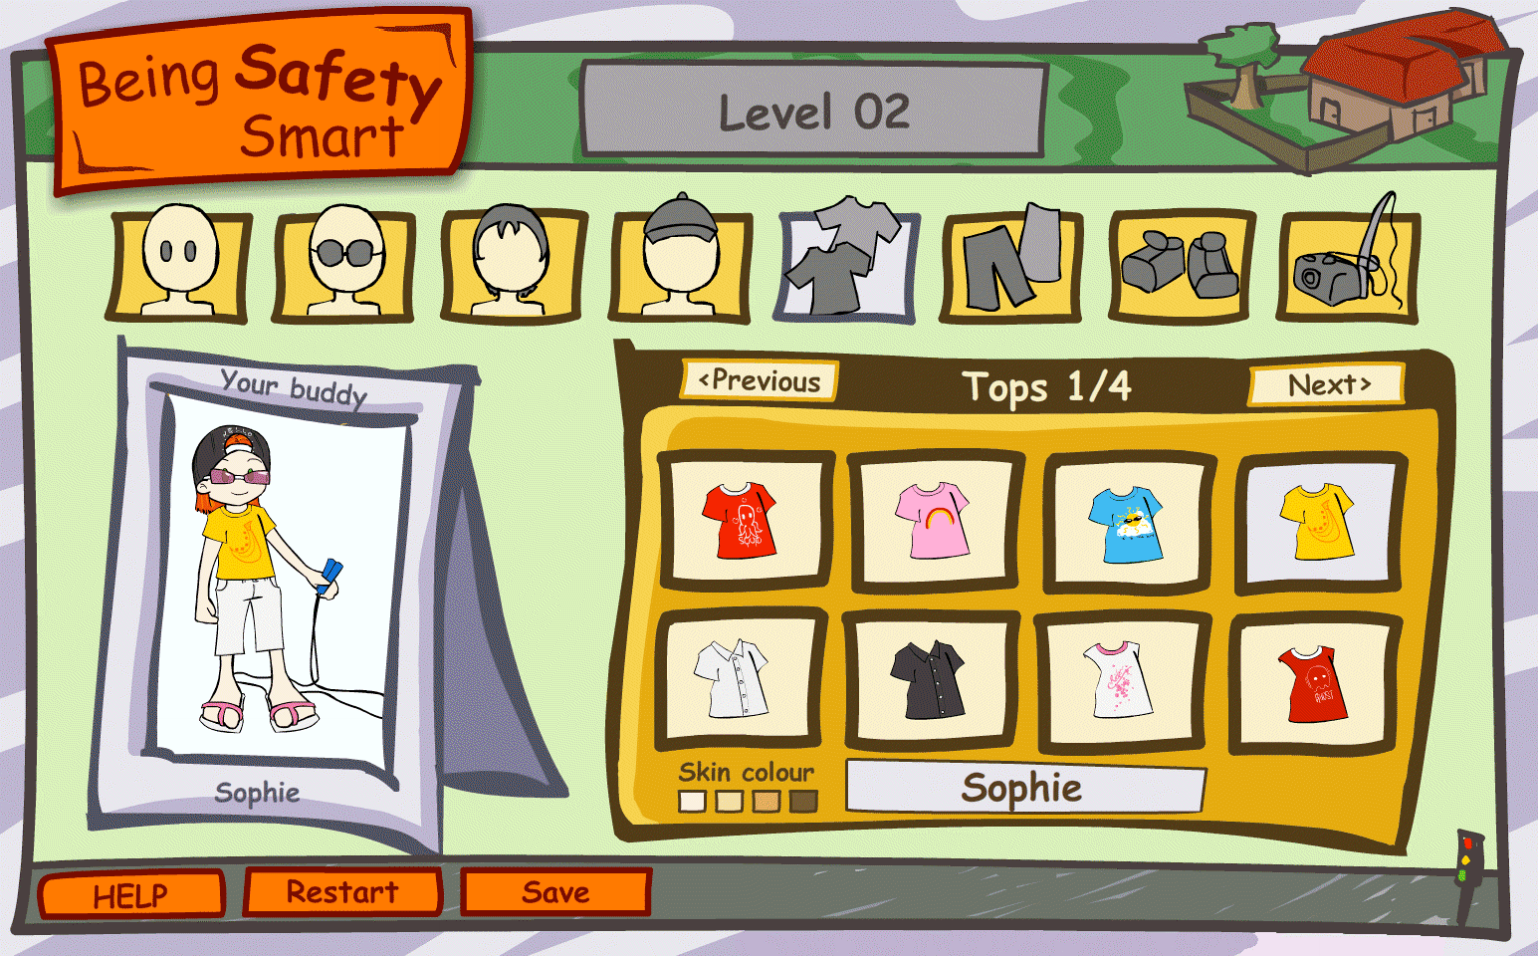
\includegraphics[width=\linewidth]{./Visuais/BSS/B2.png}}\vspace{-3pt}
  \\
  \subfloat[Nível 3.\label{fig:3}\vspace{-5pt}]{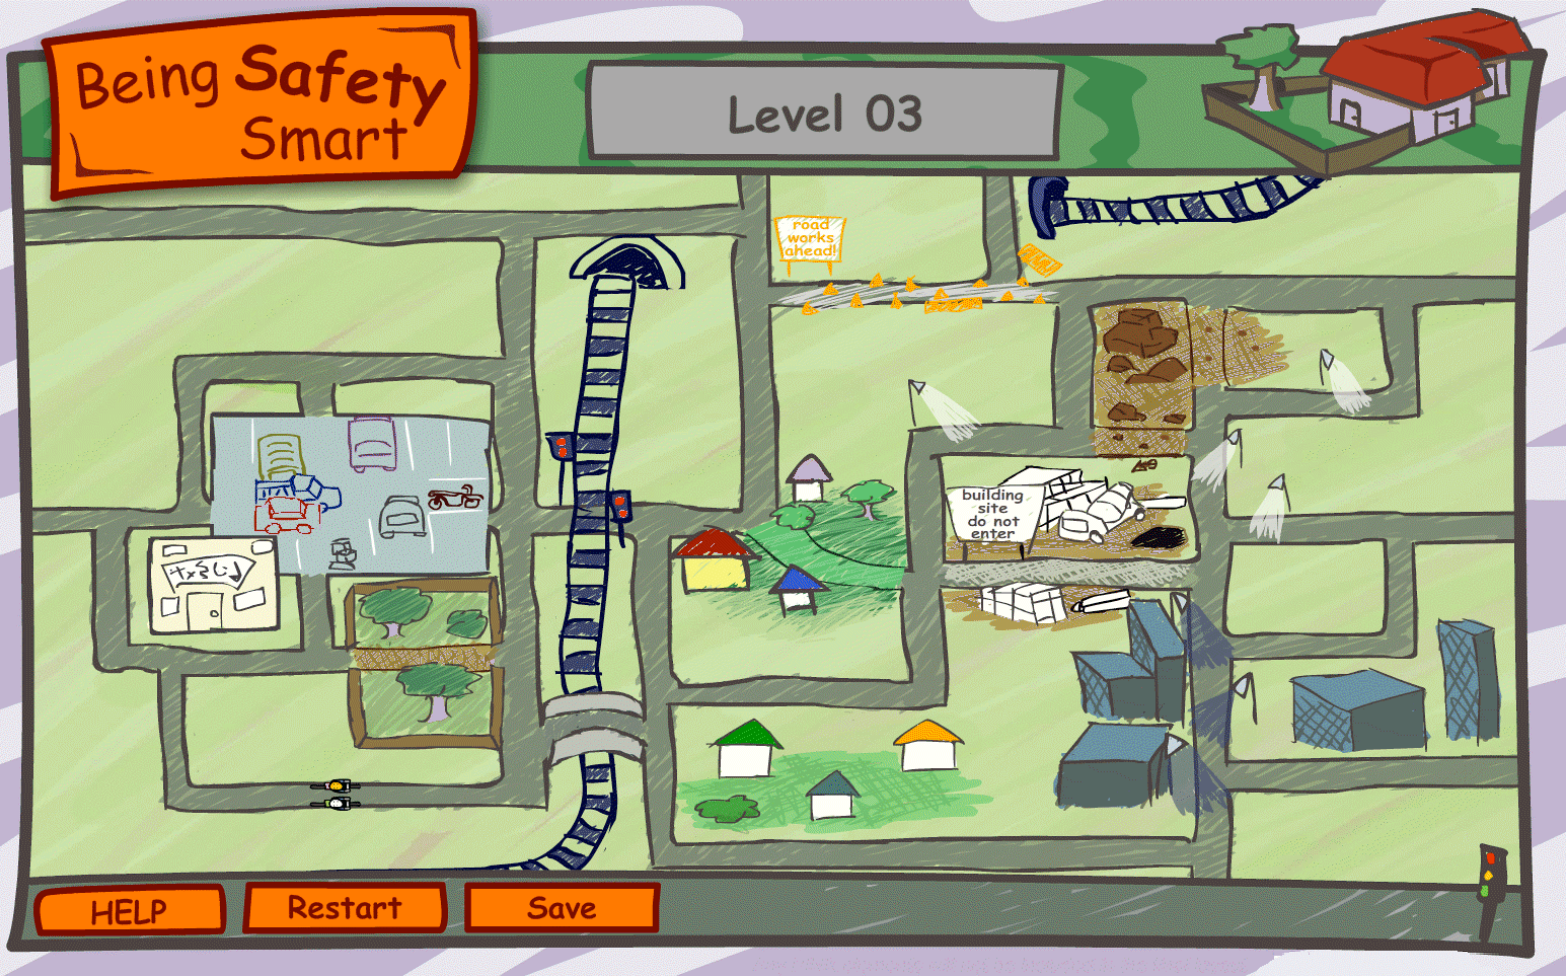
\includegraphics[width=\linewidth]{./Visuais/BSS/B8.png}}\vspace{-3pt}
  \\
  \subfloat[Nível 4.\label{fig:4}\vspace{-5pt}]{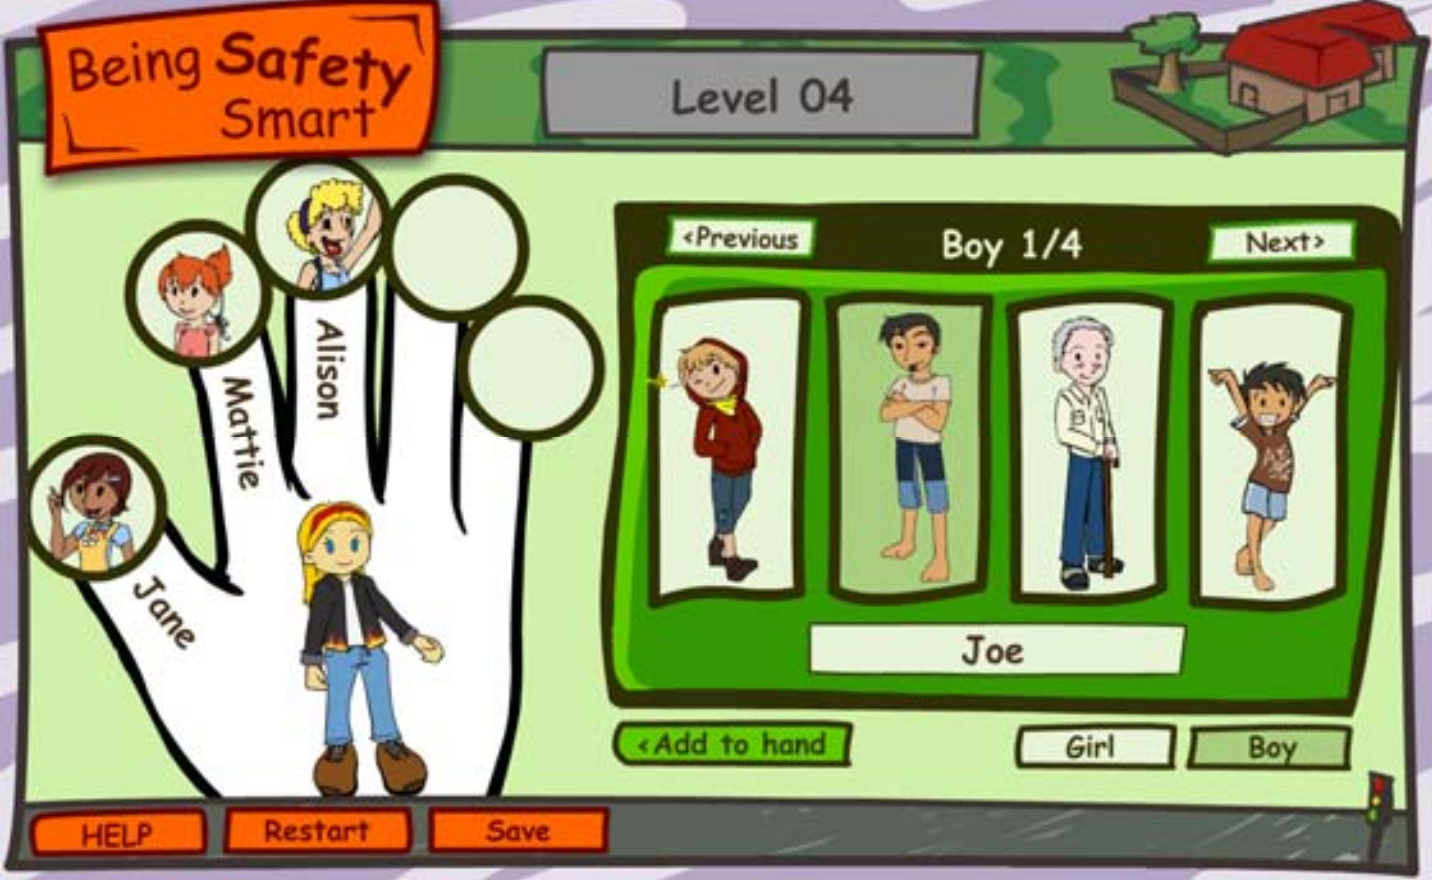
\includegraphics[width=\linewidth]{./Visuais/BSS/B9.png}}\vspace{-3pt}
  \\
  \subfloat[Nível 5.\label{fig:5}\vspace{-5pt}]{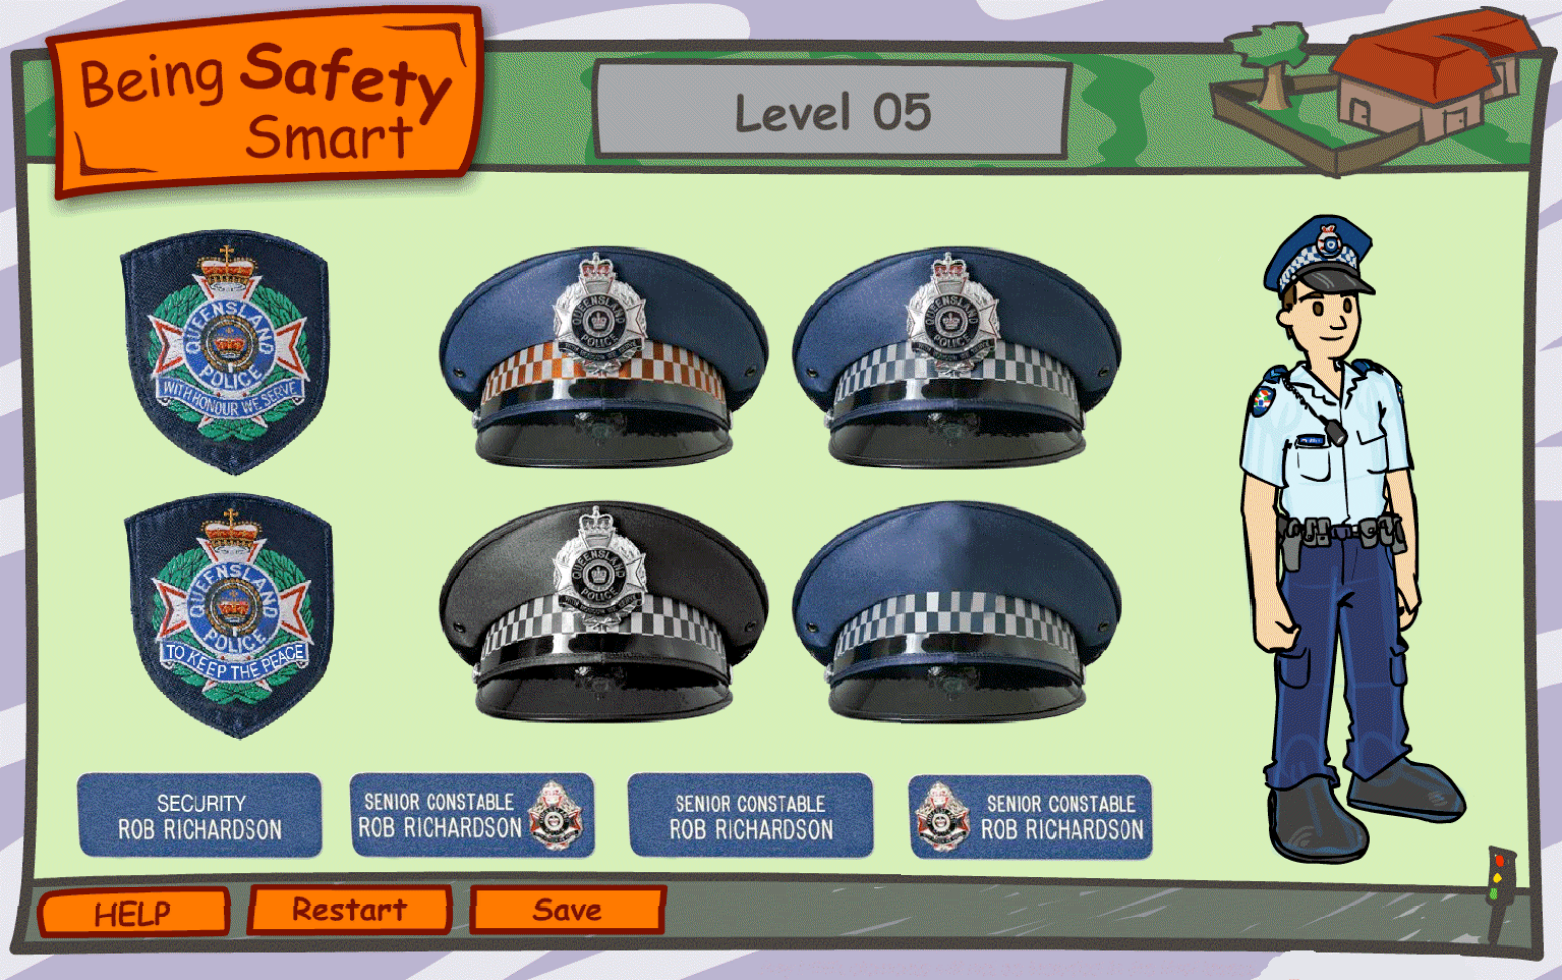
\includegraphics[width=\linewidth]{./Visuais/BSS/B6.png}}\vspace{-3pt}
  \\
  \subfloat[Nível 6.\label{fig:6}\vspace{-5pt}]{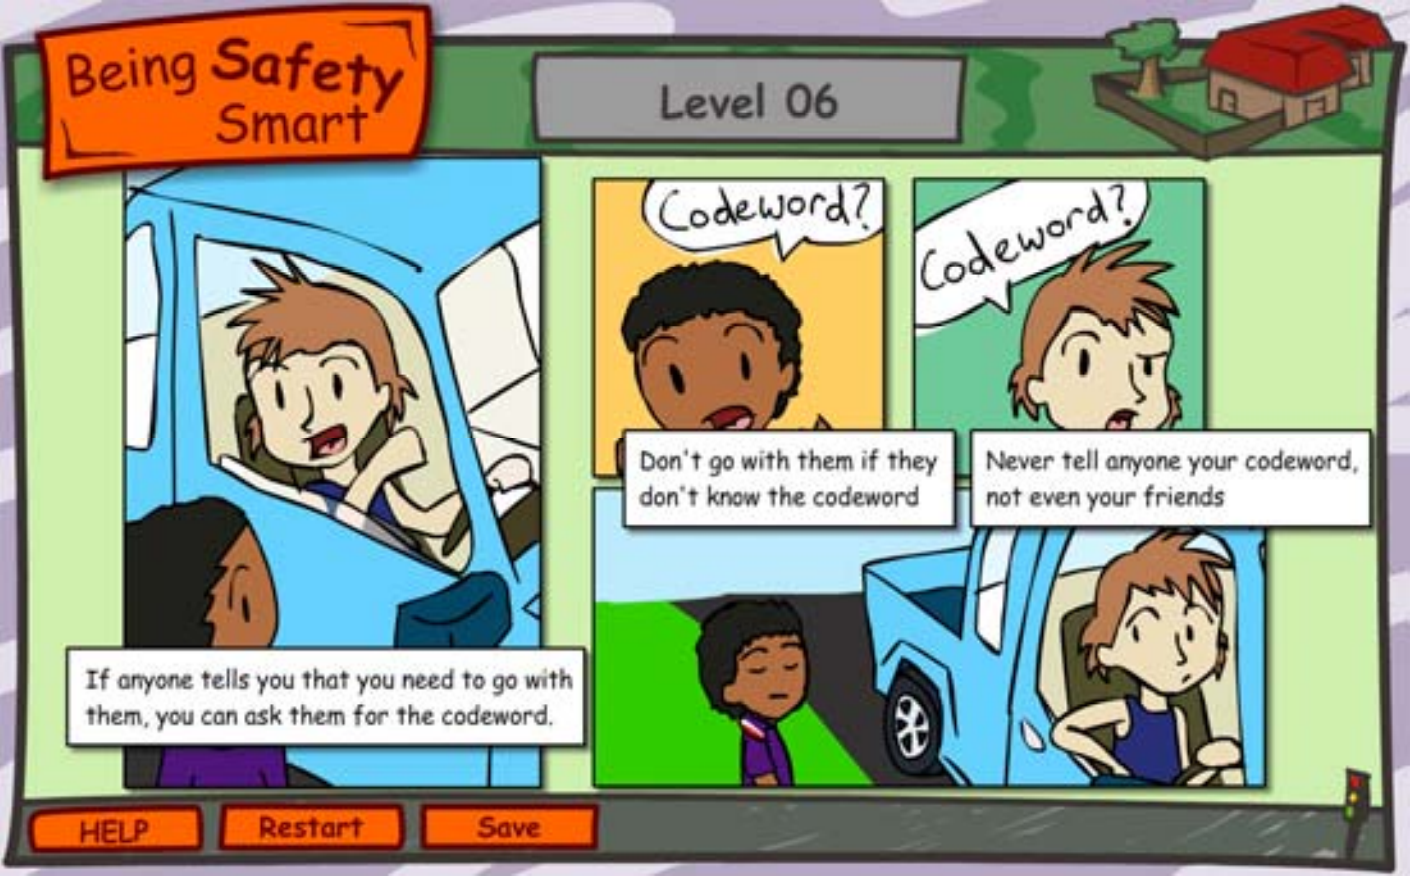
\includegraphics[width=\linewidth]{./Visuais/BSS/B10.png}}\vspace{-3pt}
  \\
  \subfloat[Nível 7.\label{fig:7}\vspace{-5pt}]{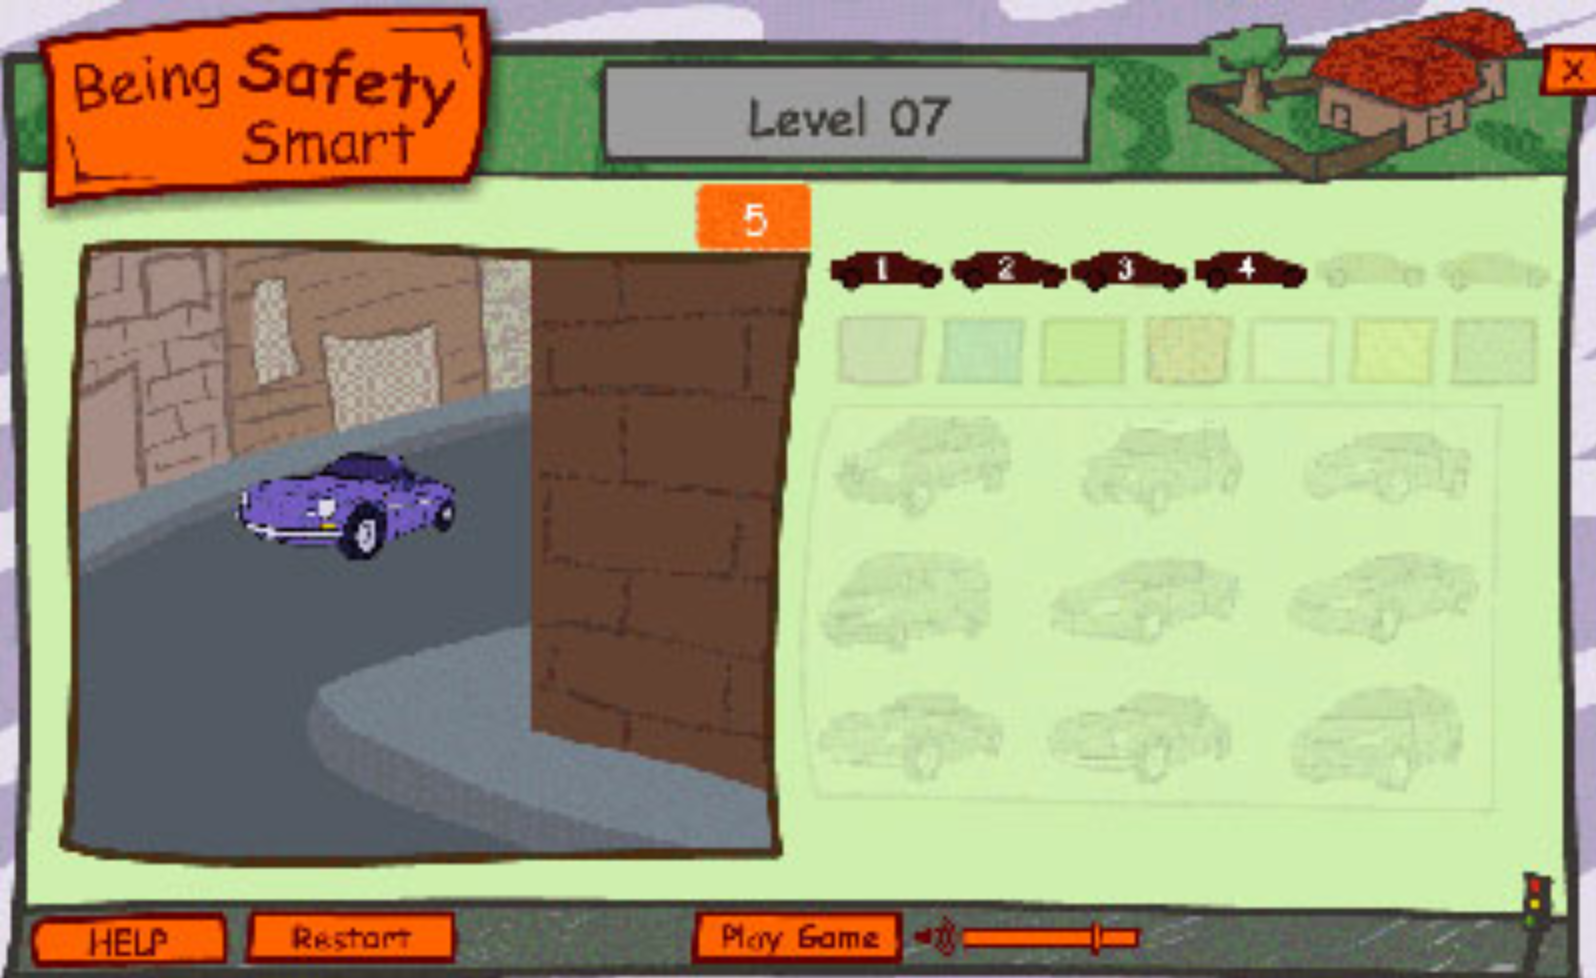
\includegraphics[width=\linewidth]{./Visuais/BSS/B12.png}}\vspace{-3pt}
  \\
  \subfloat[Nível 8.\label{fig:8}\vspace{-5pt}]{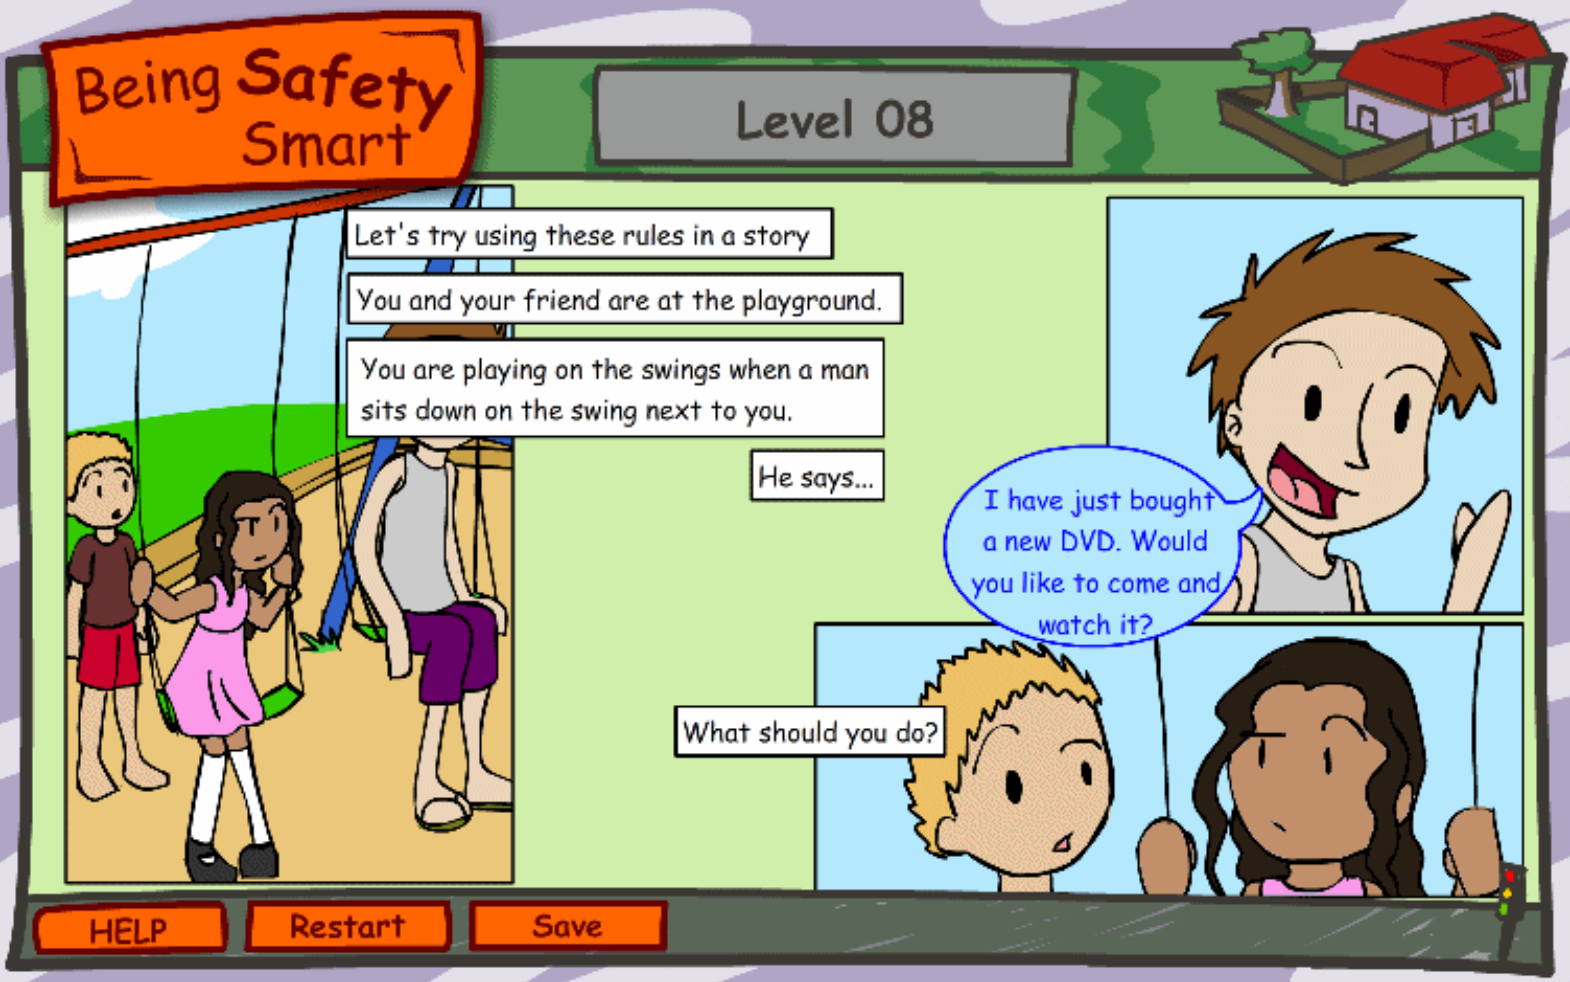
\includegraphics[width=\linewidth]{./Visuais/BSS/B11.png}}
  \vspace{-1pt}
  \legend{Fonte: \citeonline{jones2008online}.}%eu paguei outros nao citados aqui, como fazer a referencia?
  %india (mas não governamental)
\end{wrapfigure}

A numeração dos níveis representa a linearidade imposta pelo jogo ao jogador. O jogo exige um cumprimento linear dos seus níveis, tanto por motivos de enredo, quanto por motivos pedagógicos de ensino. Um jogador só pode acessar os níveis inferiores ao seu progresso no jogo. O jogador precisa esperar que a história do jogo vá destravando, um a um, os níveis superiores. Ao acessar o jogo, o jogador deve realizar um breve cadastro para ter acesso ao mapa do jogo e seus oito níveis, podendo ainda customizar seu personagem. No primeiro nível (Figura \ref{fig:1}) a criança aprende que deve sempre informar aos seus pais (ou responsáveis) os locais aonde vai e com quem vai ao sair de casa com os amigos. No segundo nível (Figura \ref{fig:2}) o jogador é ensinado a nunca andar sozinho sempre que isso for possível. No terceiro nível (Figura \ref{fig:3}) a criança é instruída a caminhar sempre por locais seguros e conhecidos. No quarto nível (Figura \ref{fig:4}) o menor aprende a reconhecer e identificar cinco adultos em quem possa confiar. No quinto nível (Figura \ref{fig:5}) o jogador é ensinado a identificar outras pessoas a quem possa pedir ajuda ou auxílio. No sexto nível (Figura \ref{fig:6}) o menor aprende a identificar pessoas confiáveis através de um sistema de contrassenha (\textit{e.g.} as contrassenhas ou \textit{codeworks} são senhas usadas entre as pessoas para reconhecerem se a outra pessoa é uma pessoa de confiança). No sétimo nível (Figura \ref{fig:7}) o jogador aprende a evitar presentes de estranhos (\textit{e.g.} evitando caronas de desconhecidos e presentes ou doces de estranhos). E no oitavo nível (Figura \ref{fig:8}) o jogo ensina ao jogador a sempre comunicar e contar para pessoas de confiança situações incomuns ou desagradáveis que tenham acontecido. 

Todos os níveis do jogo \textit{Being Safety Smart} compartilham a mesma arte baseada em quadrinhos infantis. Cada diálogo do jogo é acompanhado por texto escrito e dublagem em língua inglesa. Além disso, os níveis do jogo compartilham a mesma estrutura didática baseada em três conceitos metodológicos de ensino. Inicialmente o jogador é apresentado as instruções de um determinado nível. Posteriormente o jogador é confrontado com uma atividade lúdica interativa. E por fim, o jogador é apresentado a um resumo do nível. Os oito níveis do jogo são projetados para serem ministrados em um ambiente escolar no decorrer de 8 (oito) semanas. Contudo, nada impede que o jogo seja ofertado em blocos mais curtos ou mais longos de tempo a depender das temáticas já ministradas pela escola \cite{jones2010being}. Em adendo, a literatura revela que mais de 200 (duzentas) escolas já ministraram o jogo \textit{Being Safety Smart} a seus alunos.

O jogo \textit{Being Safety Smart} teve sua eficácia verificada por meio de um processo avaliativo \cite{jones2010being}. O processo buscou encontrar relações entre os graus de aprendizagem de uma amostra de crianças e os assuntos ministrados pelo jogo. Para se verificar essa relação, a amostra de crianças foi previamente dividida em dois grupos: um grupo controle e um grupo experimental. O grupo controle consistia do conjunto de participantes (crianças) que não jogaram o jogo. O grupo experimental, por sua vez, consistia do conjunto de participantes (crianças) que jogaram o jogo \textit{Being Safety Smart}. O processo avaliativo mediu então, os graus de aprendizagem dos participantes anteriormente (pré-teste) e posteriormente (pós-teste) aos testes com o jogo. A medicação dos graus de aprendizagem dos participantes se deu por meio do questionário \acf{CKAQ}. A ideia da etapa de pré-teste é averiguar o alinhamento no nível de conhecimento de ambos os grupos no que diz respeito aos conteúdos do questionário. Já a ideia da etapa de pós-teste é constatar diferenças significativas no nível de conhecimento entre os grupos no que diz respeito também, aos conteúdos do questionário.

A etapa da pré-teste teve a participação de 70 (setenta) crianças: 34 (trinta e quatro) do grupo controle e 36 (trinta e seis) do grupo experimental. A medição dos resultados revelou uma taxa de acerto do questionário de 67,83\% ($\sigma$ = 7,91\%) para o grupo controle e 66,11\% ($\sigma$ = 15,41\%) para o grupo experimental. Os resultados demonstram que ambos os grupos compartilhavam o mesmo nível de conhecimento na etapa de pré-teste da pesquisa \cite{jones2010being}. Após estes resultados, o grupo experimental foi convidado a jogar o jogo. Depois de jogar o jogo por 8 (oito) semanas, ambos os grupos foram convidados a responderem novamente o questionário \ac{CKAQ}. 

A etapa de pós-teste teve a participação de 76 (setenta e seis) crianças: 37 (trinta e sete) do grupo controle e 39 (trinta e nove) do grupo experimental. A medição dos resultados apresentou um percentual de acerto do questionário de 69,11\% ($\sigma$ = 10,49\%) para o grupo controle e 89,97\% ($\sigma$ = 11,18\%) para o grupo experimental. Os dados mostram uma nítida evolução no desempenho do grupo experimental em relação ao grupo controle, implicando assim, uma possível influência do jogo ministrado. Entre os jogadores, o jogo parece ser capaz de ampliar a compreensão das crianças no que diz respeito as estratégias de segurança pessoal.

Durante toda a pesquisa os profissionais envolvidos receberam treinamento adequado, sendo instruídos a proceder adequadamente a quaisquer casos de violência sexual infantil que fossem revelados no decorrer da pesquisa \cite{jones2010being}. Além disso, os responsáveis das crianças tiveram participação ativa neste processo, sendo responsáveis por notificarem qualquer alteração no comportamento das crianças como ansiedade ou angústia. O jogo então manifesta dois resultados positivos, o primeiro de ampliar os conhecimentos das crianças acerca sua segurança pessoal e o segundo pelo fato do jogo não manifestar qualquer desconforto ou mudança inadequada de comportamento aos jogadores. 

%-------------------------------------------------------------------------------------------------------------------

\section{Orbit Rescue}\label{sssec:Orbit}

\textit{Orbit Rescue}\footnote{\textit{Orbit Rescue} é um \acf{JS} desenvolvido pela Universidade de Sunshine Coast e lançado em 2012. Mais informações sobre o jogo podem ser acessadas em seu portal: \url{http://orbit.org.au/}.} é um jogo no estilo aventura projetado para conscientizar as crianças sobre a violência sexual infantil. O jogo é voltado a atender crianças entre 8 (oito) e 10 (dez) anos de idade. Dentre os ensinamentos ministrados pelo jogo estão conceitos de: privacidade corporal, comunicação, confiança e defesa pessoal. Os quatro ensinamentos se traduzem em quatro fases a serem acessadas no jogo, o qual possui texto e dublagem em inglês, apenas. A \autoref{fig:selecao} ilustra a tela de seleção de fases do jogo.

\begin{figure}[htb]
	\caption{\label{fig:selecao}Tela de seleção das fases do jogo \textit{Orbit Rescue}.}
  \begin{center}\vspace{-0.3cm}
    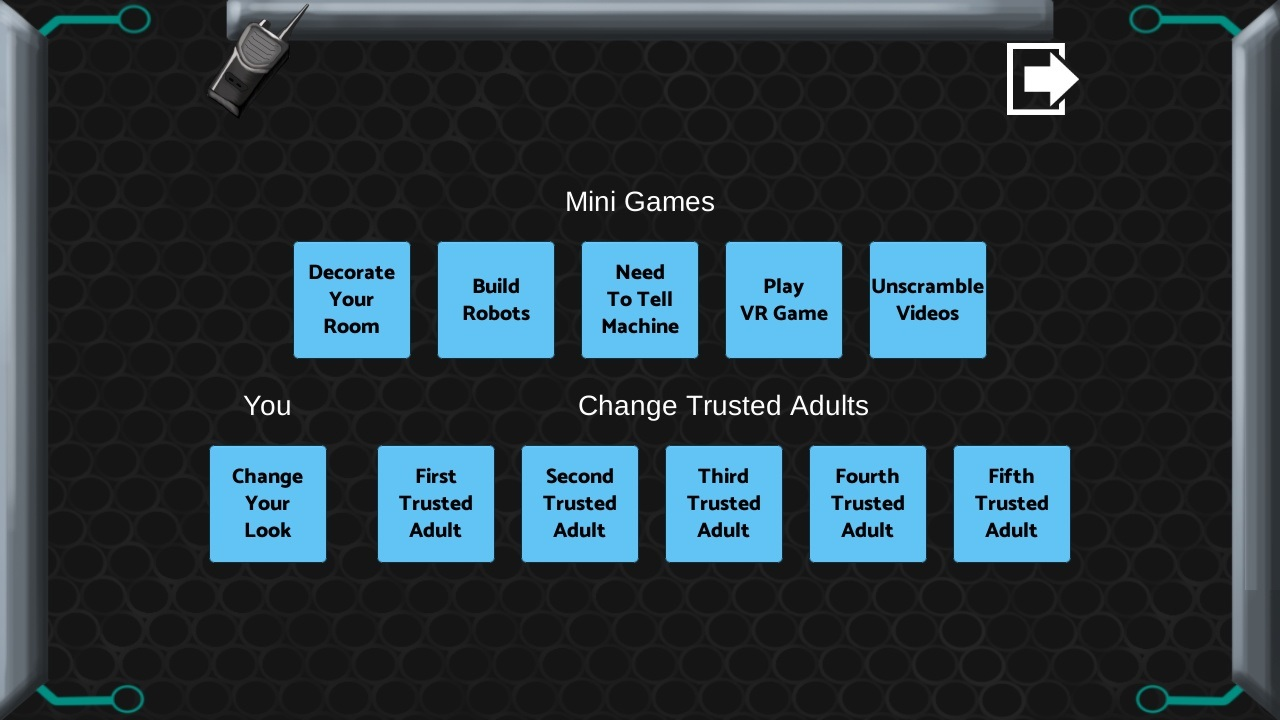
\includegraphics[width=0.92\linewidth]{./Visuais/Orbit/OrbitFases.jpg}
	\end{center}\vspace{-0.2cm}
  \legend{Fonte: \citeonline{steiler2012orbit}}
\end{figure}

\vspace{-0.3cm}


O jogo \textit{Orbit Rescue} dispõe de dois canais de acesso as fases do jogo. As fases do jogo podem ser acessadas em determinados cenários, ou podem ser acessadas por meio de um ícone que leva a uma tela de seleção de fases como mostra a \autoref{fig:selecao}. Cada fase se traduz em um minijogo com dinâmica e ensinamentos distintos entre si, cada fase contém uma quantidade variada de níveis a serem explorados. Há ainda conceitos não ministrados nos minijogos, com a questão dos adultos de confiança. Tal conceito é passado com o intuito de ensinar ao jogador a reconhecer e identificar pessoas em quem possa confiar. O jogador deve então, personificar no jogo cinco adultos de confiança. Indiretamente o jogador aprende a sempre estar acompanhado por alguém de confiança, pois o personagem fabricado acompanha o personagem do jogador em grande parte da história do jogo. Por fim, a \autoref{fig:selecao} também apresenta algumas opções que não estão associadas a um contexto pedagógico direto, como a customização do personagem ou do quarto do personagem. Por não terem significância didática, tais opções não são apresentadas nesse trabalho. 


\begin{wrapfigure}[30]{r}{5.5cm}%pulando 30 linhas
  \vspace{-5pt}
  \caption{\label{fig:orbitniveis}Níveis.\vspace{0pt}}

  \subfloat[Nível 1.\label{fig:11}\vspace{-2pt}]{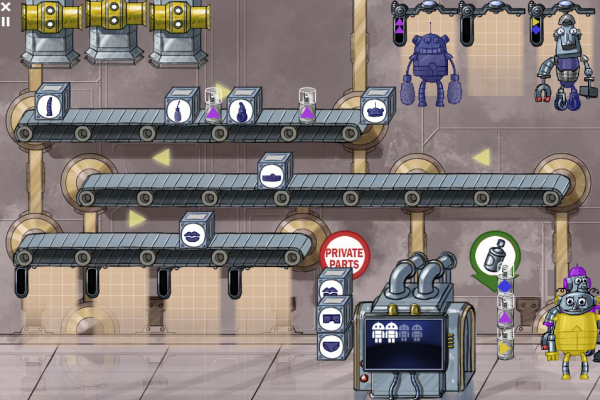
\includegraphics[width=\linewidth]{./Visuais/Orbit/robot-factory-screenshot.png}}\vspace{-0pt}
  \\
  \subfloat[Nível 2.\label{fig:22}\vspace{-2pt}]{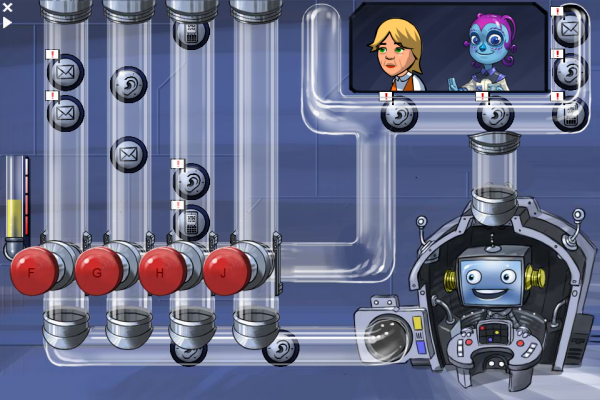
\includegraphics[width=\linewidth]{./Visuais/Orbit/need-to-tell.png}}\vspace{-0pt}
  \\
  \subfloat[Nível 3.\label{fig:33}\vspace{-2pt}]{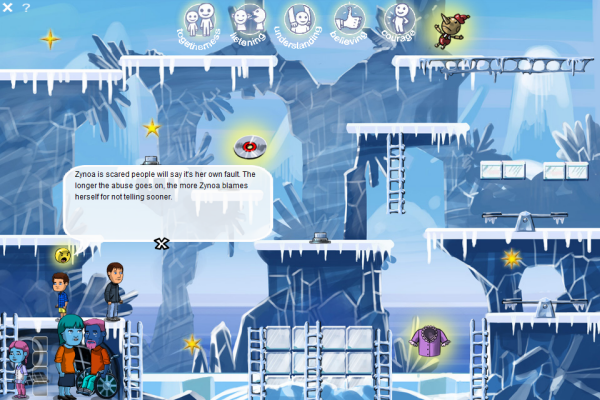
\includegraphics[width=\linewidth]{./Visuais/Orbit/speak-up.png}}\vspace{-0pt}
  \\
  \subfloat[Nível 4.\label{fig:44}\vspace{-2pt}]{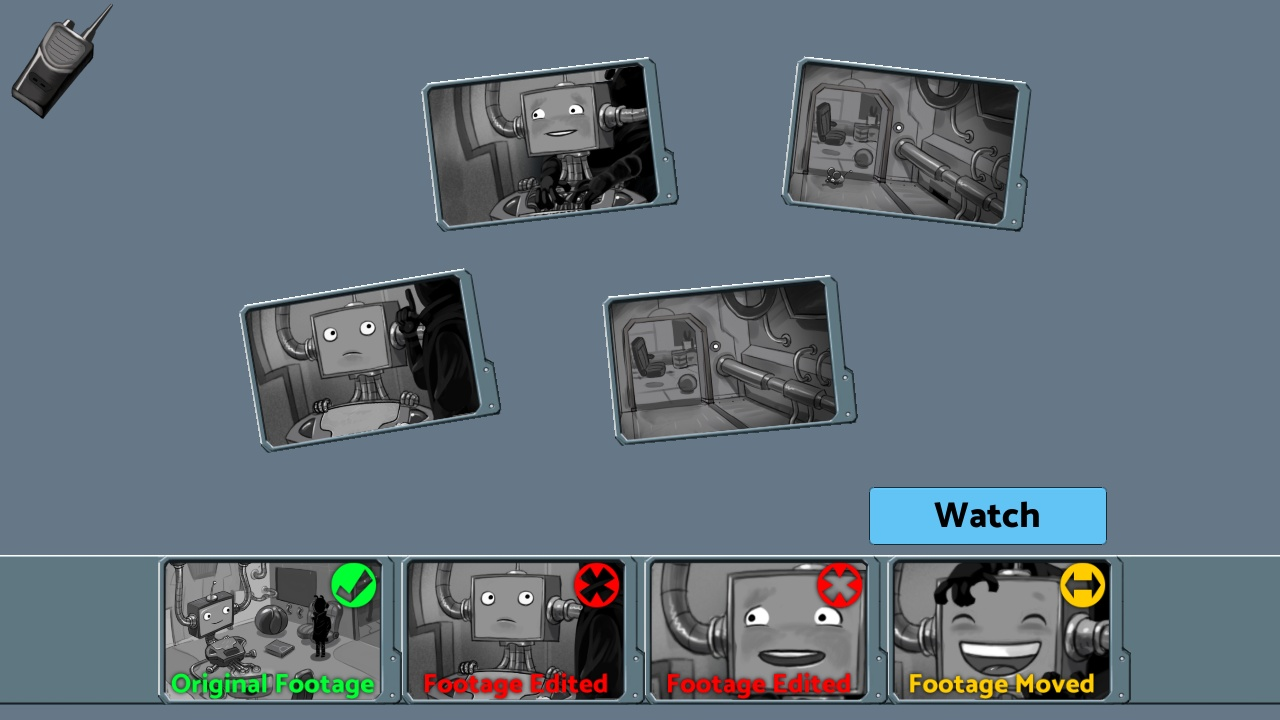
\includegraphics[width=\linewidth]{./Visuais/Orbit/cameras.jpg}}\vspace{-0pt}
  \vspace{-2pt}
  \legend{Fonte: \citeonline{steiler2012orbit}}%eu paguei outros nao citados aqui, como fazer a referencia?
  %india (mas não governamental)
\end{wrapfigure}

A \autoref{fig:orbitniveis} apresenta os quatro minijogos ministrados pelo jogo \textit{Orbit Rescue}. Cabe salientar que o jogo segue uma narrativa, por tal razão as fases não se encontram disponíveis ao jogador em um momento inicial. A ordem estabelecida na \autoref{fig:orbitniveis} representa a ordem que as fases vão sendo liberadas ao jogador. Inicialmente o jogador é ensinado sobre sua privacidade corporal (Figura \ref{fig:11}), nesta fase o jogador aprende quais são as partes íntimas e que elas não devem ser tocadas. Em seguida o jogador é ensinado a se comunicar devidamente (Figura \ref{fig:22}), o intuito desta fase é ajudar a criança a identificar situações que precisam ser reportadas para adultos de confiança. Conforme a história do jogo avança a criança aprende em um dado momento a ganhar confiança (Figura \ref{fig:33}), essa fase almeja ensinar a criança a superar episódios de abuso e a como proceder em tais situações. Por fim, em sua última fase, o jogo discorre sobre as abordagens utilizadas pelos agressores sexuais (Figura \ref{fig:44}), o jogador então deve identificar neste momento como é a atuação de um agressor sexual e aprender a reconhecer tais estratégias desde seu momento inicial e a tomar as devidas medidas. A conclusão da última fase encerra a história e a narrativa do jogo. Salienta-se nesse sentido que, embora os minijogos acompanhem o enredo do jogo, o jogador é livre para acessar qualquer uma das fases já liberadas sempre que desejar, sem quaisquer prejuízos a narrativa ou a história do jogo. 

O jogo \textit{Orbit Rescue} passou por um processo avaliativo com o intuito de averiguar o conhecimento dos jogadores sobre o abuso infantil. Para averiguar o conhecimento dos jogadores os pesquisadores utilizaram o questionário \ac{CKAQ} nas etapas de pré e pós-teste da pesquisa \cite{jones2020serious}.

O processo avaliativo durou cerca de 4 (quatro) meses. Ao total 139 (cento e trinta e nove) crianças dispersas em três grupos participaram da pesquisa. O primeiro grupo foi submetido ao jogo e a um plano de ensino. O segundo grupo foi submetido apenas ao jogo. E o terceiro grupo não foi submetido nem ao jogo nem ao plano de ensino. Na etapa de pré-teste todos os grupos beiraram uma taxa de acerto de 75\% no questionário. O mesmo resultado se manteve para o terceiro grupo na etapa de pós-teste, porém o primeiro e o segundo grupo alcançaram uma taxa de acerto no questionário de 90\%. Enfatiza-se que o primeiro grupo acertou em média, uma ou duas questões a mais no questionário em relação ao segundo grupo. A análise dos resultados revela a eficácia do jogo no que diz respeito aos conteúdos ministrados.

%Olhando individualmente, as crianças que mais obtiveram mais sucesso no questionário foram as que finalizaram o jogo, evidenciando assim, os sucesso do jogo na temática tratada.

%-------------------------------------------------------------------------------------------------------------------

\section{Cool and Safe}\label{sssec:CeS}

\textit{Cool and Safe}\footnote{\textit{Cool and Safe} é um jogo desenvolvido pela Universidade de Frankfurt lançado ao público em 2013. Mais informações sobre o jogo podem ser acessadas em seu portal: \url{https://www.coolandsafe.eu/}.} é um jogo para navegadores voltado para prevenção da violência sexual de crianças. O jogo é destinado a atender crianças na faixa dos 7 (sete) aos 12 (doze) anos. O jogo almeja prevenir a violência sexual infantil por meio da expansão do repertório comportamental das crianças, do fortalecimento de suas habilidades de autoafirmação e por meio de instruções para as crianças aprenderem a lidar com situações perigosas \cite{pajala2018compiled}. O jogo está inteiramente localizado em alemão, francês, inglês e espanhol. Todos os assuntos ministrados pelo jogo, são transmitidos as crianças por meio de texto, imagem ou vídeo em alemão, francês, inglês ou espanhol, a depender das configurações de idioma. A página inicial do portal do jogo é mostrada na \autoref{fig:portal}.

\begin{figure}[htb]

	\caption{\label{fig:portal}Portal do jogo \textit{Cool and Safe}.}
  \begin{center}%\vspace{-0.3cm}
    \includegraphics[width=\linewidth]{./Visuais/Cool/cool.png}
	\end{center}%\vspace{-0.5cm}
  \legend{Fonte: \citeonline{fingerle2012cool}}

\end{figure}

A \autoref{fig:portal} apresenta a página principal do portal do jogo \textit{Cool and Safe}. Nesta página é possível observar as opções para troca de idioma, simbolizadas pelas bandeiras da Alemanha, Reino Unido, França e Espanha. O jogo requer um cadastro para acesso, sendo necessário cadastrar um nome, senha, dia e mês de aniversário. Após o cadastro, o jogador obtém livre acesso ao jogo. Ao começar a jogar, o jogador é apresentado a vários clipes de filmes, histórias e tarefas nos quais deve ponderar e escolher entre diferentes alternativas \cite{mueller2012web}. 

\begin{wrapfigure}[30]{r}{5.5cm}%pulando 30 linhas
  \vspace{-5pt}
  \caption{\label{fig:coolniveis}Níveis.\vspace{1pt}}

  \subfloat[Nível 1.\label{fig:111}\vspace{-7pt}]{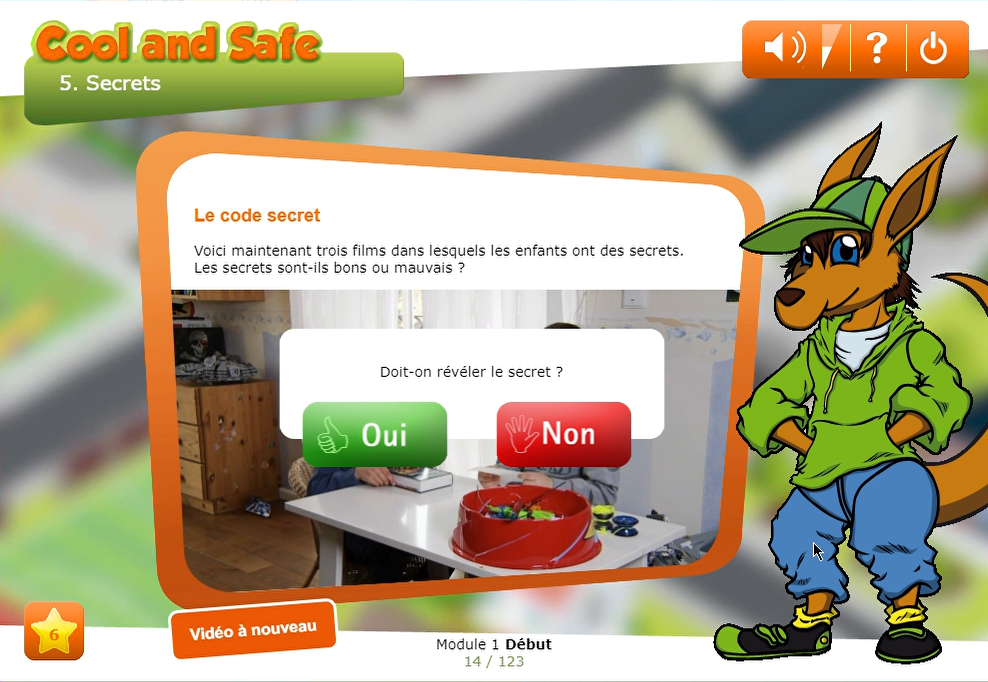
\includegraphics[width=\linewidth]{./Visuais/Cool/nivel11.png}}\vspace{-2pt}
  \\
  \subfloat[Nível 2.\label{fig:222}\vspace{-7pt}]{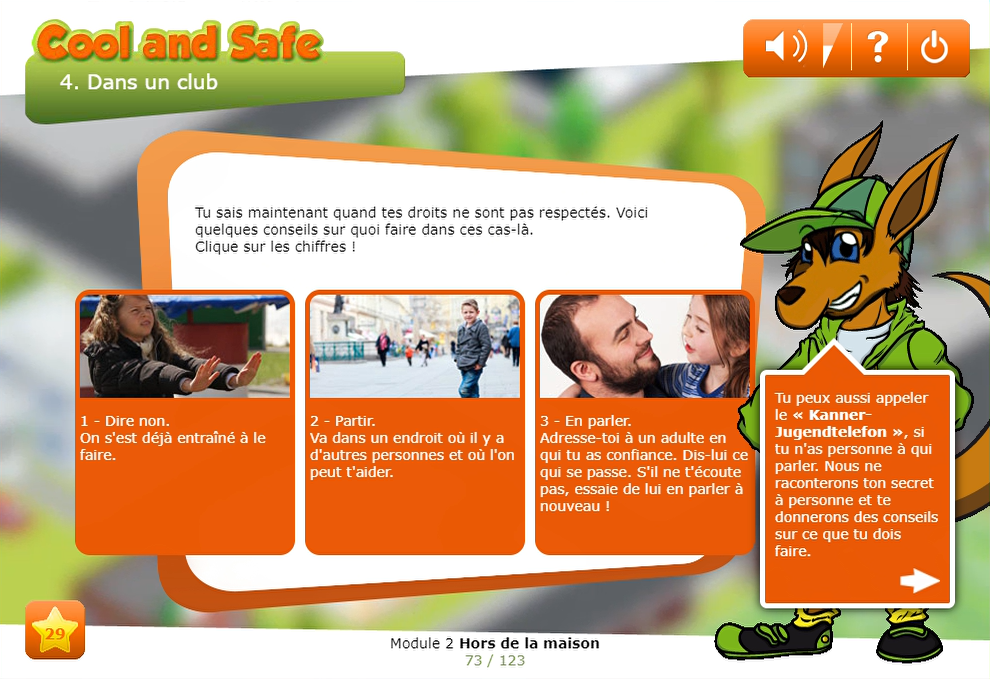
\includegraphics[width=\linewidth]{./Visuais/Cool/nivel222.png}}\vspace{-2pt}
  \\
  \subfloat[Nível 3.\label{fig:333}\vspace{-7pt}]{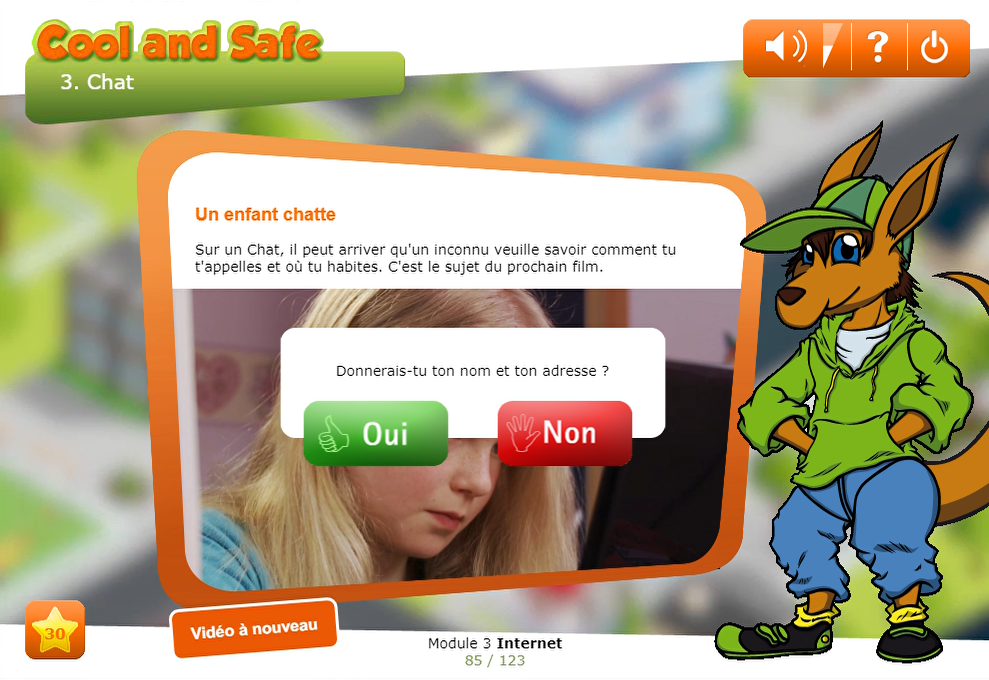
\includegraphics[width=\linewidth]{./Visuais/Cool/nivel3.png}}\vspace{-2pt}
  \\
  \subfloat[Nível 4.\label{fig:444}\vspace{-7pt}]{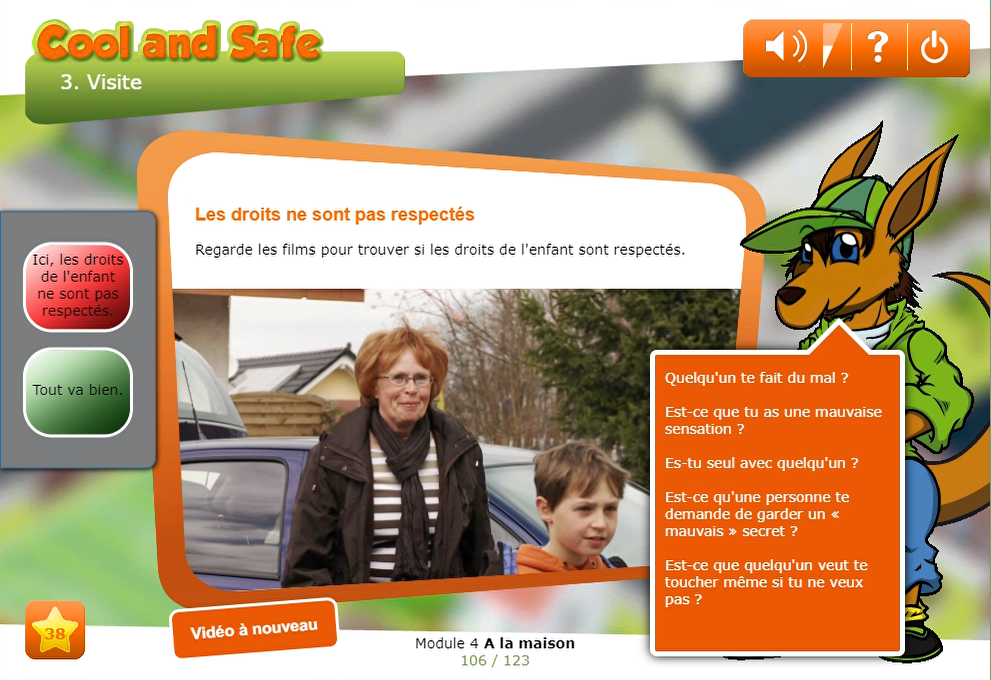
\includegraphics[width=\linewidth]{./Visuais/Cool/nivel4.png}}\vspace{-2pt}
  \vspace{-2pt}
  \legend{Fonte: \citeonline{fingerle2012abschlussbericht}}%eu paguei outros nao citados aqui, como fazer a referencia?
  %india (mas não governamental)
\end{wrapfigure}

O jogo é constituído por cinco módulos de ensinamentos para as crianças. Cada módulo corresponde a um conceito distinto a ser apreendido pelo jogador. A sequência dos módulos é fixa e não pode ser alterada. Portanto, não é possível realizar módulos individuais separadamente, além disso o jogador não possui flexibilidade para retornar para um determinado módulo após concluí-lo. O primeiro módulo (Figura \ref{fig:111}) consiste em apresentar alguns conceitos básicos ao jogador como interpretar sentimentos, guardar ou não segredos e conversar com os pais. O segundo módulo (Figura \ref{fig:222}) consiste em um tópico mais avançado voltado a educar sobre situações que podem ocorrer fora de casa como aceitar doces de estranhos, identificar situações perigosas e recusar caronas de estranhos. O terceiro módulo (Figura \ref{fig:333}) é destinado a ensinar ao jogador como usar adequadamente a \textit{internet}, neste módulo o jogador é ensinado a usar adequadamente as redes sociais, não adicionar estranhos e não ceder suas informações pessoais para terceiros. O quarto módulo (Figura \ref{fig:444}) busca educar o jogador sobre situações que podem acontecer dentro de casa, aqui a criança é ensinada sobre seus direitos e deveres, ensinada a não abrir a porta para estranhos e ensinada a denunciar a quebra de seus direitos para outras pessoas. O último módulo (sem figura representativa) apresenta uma compilação de algumas lições aprendidas nos módulos anteriores servindo como uma espécie de revisão. 

O jogo \textit{Cool and Safe} passou por um processo avaliativo, com intuito de identificar possíveis efeitos colaterais negativos associados à conclusão do jogo e sua eficácia. Ao total 286 (duzentas e oitenta e seis) crianças participaram do processo avaliativo \cite{muller2014child}. 

O processo avaliativo do jogo \textit{Cool and Safe} segmentou sua amostra de crianças em dois grupos: um grupo controle e um grupo experimental. Na etapa de pré-teste da pesquisa não se constatou diferença significativa entre os conhecimentos das crianças ao responderem o questionário \ac{CKAQ}, com ambos os grupos atingindo uma média de acerto no questionário de 61\% ($\sigma$ = 16\%). Este mesmo valor se manteve no grupo controle na etapa de pós-teste, contudo nesta etapa o grupo experimental alcançou uma taxa de 79\% ($\sigma$ = 14\%) de acerto do questionário. Os dados provam a eficácia do jogo. Além disso, testes emocionais foram realizados, os quais não identificaram quaisquer efeitos colaterais negativos manifestados pelas crianças após a conclusão do jogo, demonstrando que seu conteúdo se encontra adequado a idade ministrada. 


%-------------------------------------------------------------------------------------------------------------------

\section{Análise Comparativa}\label{sssec:finais}

Os jogos elencados neste Capítulo são uma resposta ao problema da violência sexual de crianças e de adolescentes. O estudo de tais jogos permite tanto compreender suas estruturas didático-pedagógicas, quanto os processos envolvidos na avaliação de tais jogos. Neste sentido, observou-se que o questionário \acf{CKAQ} norteia o processo avaliativo dos jogos apresentados. É importante que diferentes pesquisas atestem seus resultados acadêmicos através da utilização das mesmas métricas, para que o rigor do processo científico seja preservado. Assim, os resultados e achados entre uma pesquisa e outra ficam mais evidentes, uma vez que todas tenham se utilizado da mesma régua. A \autoref{tab-nivinv} compila os principais achados científicos dos trabalhos relacionados a essa pesquisa.


\newcolumntype{P}[1]{>{\centering\arraybackslash}p{#1}}
\newcolumntype{M}[1]{>{\centering\arraybackslash}m{#1}}
\begin{table}[htb]
\footnotesize
\renewcommand{\arraystretch}{1.5} %espaço entre as linhas
\caption[Trabalhos Relacionados.]{Trabalhos Relacionados.}
\label{tab-nivinv}
\centering
\begin{tabular}{p{4.2cm}p{2.0cm}M{2.2cm}M{1.5cm}M{2.0cm}M{2.1cm}}
  \toprule
   \textbf{Jogo (Ano)} & \textbf{Idioma}  & \textbf{Público-alvo} & \textbf{Amostra} & \multicolumn{2}{c}{\textbf{Avaliação (pós-teste)}}  \\
   \cline{5-6}
     &  &  &  & Grupo Controle & Grupo Experimental\\
   \midrule
    \textit{Being Safety Smart} (2009)  & Inglês          & 6-8 anos    & 76    & \textcolor[rgb]{0.9,0,0}{\textbf{69\%}}      & \textcolor[rgb]{0,0.6,0}{\textbf{90\%}} \\
    \hline
    \textit{Orbit Rescue} (2012)        & Inglês          & 8-10 anos   & 139    & \textcolor[rgb]{0.9,0,0}{\textbf{75\%}}      & \textcolor[rgb]{0,0.6,0}{\textbf{93\%}} \\
    \hline
    \textit{Cool and Safe} (2013)       & $\frac{Alem\tilde{a}o/Franc\hat{e}s}{Ingl\hat{e}s/Espanhol}$  & 7-12 anos   & 286   & \textcolor[rgb]{0.9,0,0}{\textbf{61\%}}      & \textcolor[rgb]{0,0.6,0}{\textbf{79\%}} \\
    \hline
    %\textit{Jogo Proposto} (2021)     & Português       & 5-8 anos    & -     &   -       &   - \\
    \bottomrule
\end{tabular}
\legend{Fonte: Elaborada pelo autor (2021).}
\end{table}


A \autoref{tab-nivinv} realiza um comparativo entre diferentes jogos voltados a prevenção da violência sexual infantil. A primeira coluna apresenta os nomes dos jogos seguido de seus anos de lançamento. A segunda coluna ilustra os idiomas nos quais os jogos encontram-se disponíveis, enfatiza-se neste sentido que todos os jogos estão localizados em seus respectivos idiomas. A terceira coluna apresenta o público-alvo dos jogos. A quarta coluna apresenta a quantidade total de participantes envolvidos no processo de avaliação de cada jogo; cabe salientar que a amostra de participantes respeitava a faixa etária estabelecida por cada jogo no que diz respeito ao seu público-alvo. Por fim, a quinta coluna apresenta os resultados e achados alcançados com amostra de participantes. 

A identificação de trabalhos relacionados é crucial para descobrir os principais métodos e processos que tange a execução de um determinado estudo \cite{wazlawick2014metodologia}. A identificação dos trabalhos relacionados a essa pesquisa, revela achados pertinentes relacionados ao seu processo de avaliação. O corrente trabalho acadêmico elenca os trabalhos relacionados com o intuito de fundamentar o processo avaliativo a ser realizado. Todavia, buscando trazer mais heterogeneidade aos trabalhos relacionados, essa pesquisa elenca também outros jogos (\autoref{sssec:outros}) que não passaram por um processo avaliativo em suas pesquisas. 

\section{Outros jogos}\label{sssec:outros}

A busca literária realizada revelou outros jogos voltados a prevenção da violência sexual infantil. Todavia, até o presente momento da redação deste trabalho não se constatou a efetiva avaliação de tais jogos com seus grupos de usuário. Desta forma, os jogos listados nessa seção não devem ser vistos como achados científicos, mas sim, como propostas de artefatos para alcançar achados científicos.

A organização \ac{ECPAT} propõe um jogo\footnote{O \acf{JS} proposto pela organização \acf{ECPAT} simula situações reais, comuns as agências de turismo. O jogo foi lançado em 2015 e possui tradução oficial em 10 (dez) idiomas. O jogo em si pode ser acessado por meio do seguinte endereço eletrônico: \url{http://www.ecpat-serious-game.eu/}.} para combater à exploração sexual de crianças e adolescentes no campo do turismo. A ideia principal do jogo é a de mobilizar as agências de turismo de modo a reforçar suas capacidades para garantir uma maior proteção das crianças. O jogo possui três etapas. Inicialmente a questão da exploração sexual de crianças é apresentada. Em seguida, o jogo instrui as agências de turismo a abordar sobre a problemática com os turistas. Por fim, o jogo ensina a proceder em cenários onde a violação de direitos de crianças tenha sido constatada \cite{gopalan2018social}. 

A empresa \textit{Mage}\footnote{\textit{Mage} é uma empresa vietnamita focada no desenvolvimento de produtos e projetos educacionais para crianças entre 2 (dois) e 12 (doze) anos de idade. Dentre os jogos produzidos pela empresa encontra-se o jogo \textit{Child Abuse Prevention} (lançado em 2018). O jogo encontra-se disponível somente na loja de aplicativos da \textit{Apple}. Mais informações sobre a empresa podem ser acessadas em sua página oficial: \url{https://mage.com.vn/}.} propõe um jogo para prevenir os maus-tratos infantis. O jogo é projetado de modo a abordar seis questões relacionadas a prevenção da violência sexual infantil. A primeira lição foca em ensinar as crianças a respeito de suas partes do corpo. A segunda lição visa educar os menores sobre toques inseguros/impróprios advindos por terceiros. A terceira lição ensina as crianças a evitarem e relatarem tentativas de abuso. A quarta lição menciona sobre toques confusos. A quinta lição aborda agressões em um contexto geral. E a sexta lição fala sobre os círculos de confiança, ensinando as crianças a quais indivíduos podem confiar.

\citeonline{carrara2018criancca} propõem um jogo para combater a violência sexual infantil a nível nacional. O jogo em si, tem o objetivo de auxiliar responsáveis e educadores a prevenirem o abuso sexual de crianças e adolescentes. Os ensinamentos do jogo são inteiramente customizáveis, permitindo aos administradores (responsáveis ou professores) a adaptação individual dos ensinamentos do jogo, proporcionando que a aprendizagem seja voltada ao indivíduo, e não, ao coletivo. Os ensinamentos do jogo são passados ao jogador por intermédio de perguntas. Cada pergunta acompanha um conjunto de respostas, as quais, o jogador deve ponderar de modo a identificar a resposta mais apropriada a uma determinada pergunta, sendo portanto, um jogo de perguntas e respostas. Há um cronometro que acompanha cada pergunta, sendo assim, a quantidade de erros, acertos e tempo de resposta de cada jogador compõem sua pontuação final no jogo. Por ser inteiramente customizável, não há uma estrutura pedagógica que possa ser apontada. Sendo assim, cabe aos administradores, ponderar e eleger os principais conceitos que devem ser ministrados no jogo.

\citeonline{diocesano2018infancia} propõe o jogo \textbf{Infância Segura} para combater a violência sexual infantil. O jogo é destinado a atender crianças a partir dos 5 (cinco) anos de idade. No total, 4 (quatro) conceitos pedagógicos são ministrados pelo jogo no decorrer de 4 (quatro) fases. A primeira fase busca ensinar as crianças sobre suas partes do corpo. A segunda fase almeja educar os menores sobre toques ruins/impróprios advindos por terceiros. A terceira fase objetiva-se a ensinar sobre questões de comportamento social. Já a quarta fase busca ensinar as crianças questões de comportamento digital. A progressão de fases no jogo ocorre de forma linear, impossibilitando o jogador de pular fases ou até mesmo de regressar as fases já concluídas. 

O jogo \textbf{Infância Segura} é proposto não apenas como uma ferramenta de ensino, mas também como uma ferramenta de apoio e suporte para professores. Sendo assim, o jogo assume características similares a de um \ac{AVA}. A ferramenta de apoio possibilita que professores possam acessar relatórios específicos de desempenho de cada jogador no jogo, acessando informações como: quantidade de acertos e quantidade de erros. Tais relatórios permitem que os professores possam constatar indícios de violência sexual. Para auxiliar os professores nesse sentido, o jogo também fornece materiais de apoio sobre a violência sexual infantil, ajudando-os assim, a proceder em casos suspeitos de violência sexual infantil.

%O presente estudo acadêmico busca combater a violência sexual de crianças e adolescentes. Sendo assim, elencar as soluções já existentes neste cenário (\autoref{ch:Relacionados}), possibilita identificar os principais meios de atuação para se combater o problema da violência sexual infantil. Cada solução de combate ao problema ergue uma camada de defesa na proteção dos direitos das crianças e dos adolescentes. O Brasil possui excelentes políticas públicas de protenção aos direitos de crianças e adolescentes. Todavia, o Brasil ainda possui lacunas a serem preenchidas. No que diz respeito ao combate a violência sexual infantil, o Brasil carrece de um programa educacional voltado a ensinar crianças a se previnirem da violência sexual infantil. Desta forma, o presente estudo surge de modo a tentar preencer essa lacuna.

Jogos para prevenção da violência sexual infantil manifestam-se como uma excelente política pública de proteção aos direitos das crianças e dos adolescentes. O Brasil possui excelentes políticas públicas de proteção aos direitos dos menores. Todavia, o Brasil carece de uma abordagem lúdico-educativa focada em prevenir a violência sexual infantil. Ou seja, o Brasil possui uma lacuna na defesa dos direitos das crianças e dos adolescentes. Almejando garantir uma melhor defesa dos direitos das crianças e dos adolescentes o presente estudo se propõe a desenvolver e avaliar um jogo lúdico-educativo de temática preventiva a violência sexual. 

Todos os jogos listados nessa seção visam combater a violência sexual de crianças e adolescentes por meio de uma abordagem lúdico-educativa. No entanto, ao que a literatura pesquisada indica, nenhum dos jogos elencado nesta seção possui eficácia confirmada no que diz respeito ao combate à violência sexual infantil. A busca literária por tais jogos vem então com o intuito de identificar propostas promissoras de jogos para se combater a violência sexual infantil. Todavia, para se atestar isso, é necessário que um processo sistemático de avaliação seja devidamente conduzido. Dentre os jogos apresentados, acredita-se que um jogo nacional devidamente harmonizado com a realidade brasileira possui maiores chances de sucesso, frente a importação de um jogo estrangeiro. Por tal razão, o presente estudo descartou a possibilidade de adaptar ao português jogos estrangeiros voltados a prevenção da violência sexual infantil. Dentre as propostos nacionais de jogos, a corrente pesquisa elege o jogo \textbf{Infância Segura} para ser desenvolvido e implementado como proposta educativa e preventiva sobre a questão da violência sexual de crianças. O jogo em questão, destaca-se por possuir uma quantidade superior de conceitos e uma maior variedade de mecânicas em comparação aos outros jogos listados. Por tal razão, o jogo proposto por \citeonline{diocesano2018infancia} é o jogo eleito pelo corrente trabalho para ser desenvolvido e cientificamente avaliado.